% Options for packages loaded elsewhere
\PassOptionsToPackage{unicode}{hyperref}
\PassOptionsToPackage{hyphens}{url}
\PassOptionsToPackage{dvipsnames,svgnames,x11names}{xcolor}
%
\documentclass[
  12pt,
  a4paper,
]{article}
\usepackage{amsmath,amssymb}
\usepackage{lmodern}
\usepackage{setspace}
\usepackage{iftex}
\ifPDFTeX
  \usepackage[T1]{fontenc}
  \usepackage[utf8]{inputenc}
  \usepackage{textcomp} % provide euro and other symbols
\else % if luatex or xetex
  \usepackage{unicode-math}
  \defaultfontfeatures{Scale=MatchLowercase}
  \defaultfontfeatures[\rmfamily]{Ligatures=TeX,Scale=1}
\fi
% Use upquote if available, for straight quotes in verbatim environments
\IfFileExists{upquote.sty}{\usepackage{upquote}}{}
\IfFileExists{microtype.sty}{% use microtype if available
  \usepackage[]{microtype}
  \UseMicrotypeSet[protrusion]{basicmath} % disable protrusion for tt fonts
}{}
\makeatletter
\@ifundefined{KOMAClassName}{% if non-KOMA class
  \IfFileExists{parskip.sty}{%
    \usepackage{parskip}
  }{% else
    \setlength{\parindent}{0pt}
    \setlength{\parskip}{6pt plus 2pt minus 1pt}}
}{% if KOMA class
  \KOMAoptions{parskip=half}}
\makeatother
\usepackage{xcolor}
\usepackage[left=2.54cm,right=2.54cm,top=2.54cm,bottom=2.54cm]{geometry}
\usepackage{color}
\usepackage{fancyvrb}
\newcommand{\VerbBar}{|}
\newcommand{\VERB}{\Verb[commandchars=\\\{\}]}
\DefineVerbatimEnvironment{Highlighting}{Verbatim}{commandchars=\\\{\}}
% Add ',fontsize=\small' for more characters per line
\usepackage{framed}
\definecolor{shadecolor}{RGB}{248,248,248}
\newenvironment{Shaded}{\begin{snugshade}}{\end{snugshade}}
\newcommand{\AlertTok}[1]{\textcolor[rgb]{0.94,0.16,0.16}{#1}}
\newcommand{\AnnotationTok}[1]{\textcolor[rgb]{0.56,0.35,0.01}{\textbf{\textit{#1}}}}
\newcommand{\AttributeTok}[1]{\textcolor[rgb]{0.77,0.63,0.00}{#1}}
\newcommand{\BaseNTok}[1]{\textcolor[rgb]{0.00,0.00,0.81}{#1}}
\newcommand{\BuiltInTok}[1]{#1}
\newcommand{\CharTok}[1]{\textcolor[rgb]{0.31,0.60,0.02}{#1}}
\newcommand{\CommentTok}[1]{\textcolor[rgb]{0.56,0.35,0.01}{\textit{#1}}}
\newcommand{\CommentVarTok}[1]{\textcolor[rgb]{0.56,0.35,0.01}{\textbf{\textit{#1}}}}
\newcommand{\ConstantTok}[1]{\textcolor[rgb]{0.00,0.00,0.00}{#1}}
\newcommand{\ControlFlowTok}[1]{\textcolor[rgb]{0.13,0.29,0.53}{\textbf{#1}}}
\newcommand{\DataTypeTok}[1]{\textcolor[rgb]{0.13,0.29,0.53}{#1}}
\newcommand{\DecValTok}[1]{\textcolor[rgb]{0.00,0.00,0.81}{#1}}
\newcommand{\DocumentationTok}[1]{\textcolor[rgb]{0.56,0.35,0.01}{\textbf{\textit{#1}}}}
\newcommand{\ErrorTok}[1]{\textcolor[rgb]{0.64,0.00,0.00}{\textbf{#1}}}
\newcommand{\ExtensionTok}[1]{#1}
\newcommand{\FloatTok}[1]{\textcolor[rgb]{0.00,0.00,0.81}{#1}}
\newcommand{\FunctionTok}[1]{\textcolor[rgb]{0.00,0.00,0.00}{#1}}
\newcommand{\ImportTok}[1]{#1}
\newcommand{\InformationTok}[1]{\textcolor[rgb]{0.56,0.35,0.01}{\textbf{\textit{#1}}}}
\newcommand{\KeywordTok}[1]{\textcolor[rgb]{0.13,0.29,0.53}{\textbf{#1}}}
\newcommand{\NormalTok}[1]{#1}
\newcommand{\OperatorTok}[1]{\textcolor[rgb]{0.81,0.36,0.00}{\textbf{#1}}}
\newcommand{\OtherTok}[1]{\textcolor[rgb]{0.56,0.35,0.01}{#1}}
\newcommand{\PreprocessorTok}[1]{\textcolor[rgb]{0.56,0.35,0.01}{\textit{#1}}}
\newcommand{\RegionMarkerTok}[1]{#1}
\newcommand{\SpecialCharTok}[1]{\textcolor[rgb]{0.00,0.00,0.00}{#1}}
\newcommand{\SpecialStringTok}[1]{\textcolor[rgb]{0.31,0.60,0.02}{#1}}
\newcommand{\StringTok}[1]{\textcolor[rgb]{0.31,0.60,0.02}{#1}}
\newcommand{\VariableTok}[1]{\textcolor[rgb]{0.00,0.00,0.00}{#1}}
\newcommand{\VerbatimStringTok}[1]{\textcolor[rgb]{0.31,0.60,0.02}{#1}}
\newcommand{\WarningTok}[1]{\textcolor[rgb]{0.56,0.35,0.01}{\textbf{\textit{#1}}}}
\usepackage{longtable,booktabs,array}
\usepackage{calc} % for calculating minipage widths
% Correct order of tables after \paragraph or \subparagraph
\usepackage{etoolbox}
\makeatletter
\patchcmd\longtable{\par}{\if@noskipsec\mbox{}\fi\par}{}{}
\makeatother
% Allow footnotes in longtable head/foot
\IfFileExists{footnotehyper.sty}{\usepackage{footnotehyper}}{\usepackage{footnote}}
\makesavenoteenv{longtable}
\setlength{\emergencystretch}{3em} % prevent overfull lines
\providecommand{\tightlist}{%
  \setlength{\itemsep}{0pt}\setlength{\parskip}{0pt}}
\setcounter{secnumdepth}{-\maxdimen} % remove section numbering
\newlength{\cslhangindent}
\setlength{\cslhangindent}{1.5em}
\newlength{\csllabelwidth}
\setlength{\csllabelwidth}{3em}
\newlength{\cslentryspacingunit} % times entry-spacing
\setlength{\cslentryspacingunit}{\parskip}
\newenvironment{CSLReferences}[2] % #1 hanging-ident, #2 entry spacing
 {% don't indent paragraphs
  \setlength{\parindent}{0pt}
  % turn on hanging indent if param 1 is 1
  \ifodd #1
  \let\oldpar\par
  \def\par{\hangindent=\cslhangindent\oldpar}
  \fi
  % set entry spacing
  \setlength{\parskip}{#2\cslentryspacingunit}
 }%
 {}
\usepackage{calc}
\newcommand{\CSLBlock}[1]{#1\hfill\break}
\newcommand{\CSLLeftMargin}[1]{\parbox[t]{\csllabelwidth}{#1}}
\newcommand{\CSLRightInline}[1]{\parbox[t]{\linewidth - \csllabelwidth}{#1}\break}
\newcommand{\CSLIndent}[1]{\hspace{\cslhangindent}#1}
\ifLuaTeX
\usepackage[bidi=basic]{babel}
\else
\usepackage[bidi=default]{babel}
\fi
\babelprovide[main,import]{english}
% get rid of language-specific shorthands (see #6817):
\let\LanguageShortHands\languageshorthands
\def\languageshorthands#1{}
\usepackage{titling}
\pretitle{\begin{center}\LARGE
\includegraphics[width=7cm]{../img/logo_isuc.png}\\[\bigskipamount]}
\posttitle{\end{center}}
\usepackage{times}
\usepackage{caption}
\usepackage{floatrow}
\usepackage{float}
\floatsetup[figure]{capposition=top}
\floatsetup[table]{capposition=top}
\floatplacement{figure}{H}
\floatplacement{table}{h}
\usepackage{graphicx}
\usepackage{booktabs}
\usepackage{longtable}
\usepackage{array}
\usepackage{multirow}
\usepackage{wrapfig}
\usepackage{colortbl}
\usepackage{pdflscape}
\usepackage{tabu}
\usepackage{fancyhdr}
\fancyhead{}
\usepackage{threeparttable}
\usepackage{booktabs}
\usepackage{longtable}
\usepackage{array}
\usepackage{multirow}
\usepackage{wrapfig}
\usepackage{float}
\usepackage{colortbl}
\usepackage{pdflscape}
\usepackage{tabu}
\usepackage{threeparttable}
\usepackage{threeparttablex}
\usepackage[normalem]{ulem}
\usepackage{makecell}
\usepackage{xcolor}
\ifLuaTeX
  \usepackage{selnolig}  % disable illegal ligatures
\fi
\IfFileExists{bookmark.sty}{\usepackage{bookmark}}{\usepackage{hyperref}}
\IfFileExists{xurl.sty}{\usepackage{xurl}}{} % add URL line breaks if available
\urlstyle{same} % disable monospaced font for URLs
\hypersetup{
  pdflang={en},
  colorlinks=true,
  linkcolor={DarkSlateBlue},
  filecolor={Maroon},
  citecolor={Blue},
  urlcolor={DarkSlateBlue},
  pdfcreator={LaTeX via pandoc}}

\title{\vspace{5cm} Guía N°3}
\usepackage{etoolbox}
\makeatletter
\providecommand{\subtitle}[1]{% add subtitle to \maketitle
  \apptocmd{\@title}{\par {\large #1 \par}}{}{}
}
\makeatother
\subtitle{Análisis de Datos Multinivel - SOL3051}
\author{~Estudiante \href{mailto:alaffertt@estudiante.uc.cl}{Andreas Laffert}\\
\hspace*{0.333em}Profesora Camila Ortiz\\
Ayudante Andrés González\\
\vspace{8cm}}
\date{domingo 17, noviembre 2024}

\begin{document}
\maketitle

\setstretch{1.15}
\pagebreak

\hypertarget{enunciado-1}{%
\section{Enunciado 1}\label{enunciado-1}}

Analice la estructura de los datos y evalúe cual es la mejor forma de anidamiento para modelar la preocupación por la desigualdad (concern), tomando en consideración a los encuestados, encuestas, países y años. Desarrolle los cálculos y/o tests que considere necesarios. Reporte sus resultados, interprételos y concluya (4 puntos)

En vista de que la base de datos posee una estructura de encuestas longitudinales comparativas, este trabajo sigue las recomendaciones de Schmidt-Catran y Fairbrother (\protect\hyperlink{ref-schmidt-catranRandomEffectsMultilevel2016}{2016}) para definir la estructura de efectos aleatorios en el modelado de la preocupación por la desigualdad. De acuerdo con los autores, el aumento de las encuestas comparativas entre países en los últimos años ha abierto una posibilidad para la investigación comparada de estimar el efecto no solo aquellas características transversales de los países (ej. las estructuras institucionales), sino también de aquellas que varían en el tiempo dentro de los países (ej. el desempleo). En el caso de estudios longitudinales comparativos, los autores recomiendan incluir efectos aleatorios en todos aquellos niveles donde se incorporen efectos fijos, ya que omitir alguno de estos efectos en cualquier nivel jerárquico puede resultar en errores estándar subestimados y grados de libertad inflados artificialmente, lo que trae por consecuencia una mayor posibilidad de cometer error tipo I (\protect\hyperlink{ref-schmidt-catranRandomEffectsMultilevel2016}{Schmidt-Catran \& Fairbrother, 2016, p. 24}).

\begin{table}[h!]
\begin{center}
\scalebox{0.8}{
\begin{threeparttable}
\begin{tabular}{l c c c c c c}
\toprule
 & Modelo (A) & Modelo (B) & Modelo (C) & Modelo (D) & Modelo (E) & Modelo (F) \\
\midrule
Intercepto                     & $78.75^{***}$ & $78.64^{***}$ & $78.75^{***}$ & $78.68^{***}$ & $76.54^{***}$ & $77.75^{***}$ \\
                               & $(1.39)$      & $(1.72)$      & $(1.39)$      & $(1.69)$      & $(2.80)$      & $(2.16)$      \\
\midrule
AIC                            & $380017.45$   & $380693.67$   & $380019.45$   & $380012.68$   & $380381.37$   & $380014.10$   \\
BIC                            & $380043.37$   & $380719.58$   & $380054.01$   & $380047.24$   & $380415.93$   & $380057.29$   \\
Log Likelihood                 & $-190005.73$  & $-190343.83$  & $-190005.73$  & $-190002.34$  & $-190186.68$  & $-190002.05$  \\
Num. obs.                      & $41739$       & $41739$       & $41739$       & $41739$       & $41739$       & $41739$       \\
Num. groups: country\_wave     & $40$          & $$            & $40$          & $40$          & $$            & $40$          \\
Var: country\_wave (Intercept) & $77.26$       & $$            & $77.26$       & $28.20$       & $$            & $22.10$       \\
Var: Residual                  & $524.22$      & $533.57$      & $524.22$      & $524.22$      & $529.41$      & $524.22$      \\
Num. groups: country           & $$            & $26$          & $$            & $26$          & $26$          & $26$          \\
Var: country (Intercept)       & $$            & $76.57$       & $$            & $52.85$       & $83.78$       & $60.47$       \\
Num. groups: wave              & $$            & $$            & $3$           & $$            & $3$           & $3$           \\
Var: wave (Intercept)          & $$            & $$            & $0.00$        & $$            & $13.67$       & $4.19$        \\
\bottomrule
\end{tabular}
\begin{tablenotes}[flushleft]
\scriptsize{\item Nota: Celdas contienen coeficientes de regresión con errores estándares entre paréntesis. $^{***}p<0.001$; $^{**}p<0.01$; $^{*}p<0.05$. Modelo (A) = Country-Year, Modelo (B) = Country, Modelo (C) = Year/Country-Year, Modelo (D) = Country/Country-Year, Modelo (E) = Country/Year, Modelo (F) = Country/Year/Country-Year \\ \item Fuente: Elaboración propia en base a datos de Mijs (2019).}
\end{tablenotes}
\end{threeparttable}
}
\caption{\label{tab:table1} Modelos multinivel nulos para preocupación por la desigualdad con diferentes estructuras de efectos aleatorios}
\label{table:coefficients}
\end{center}
\end{table}

Como sugieren Schmidt-Catran \& Fairbrother (\protect\hyperlink{ref-schmidt-catranRandomEffectsMultilevel2016}{2016}), las principales omisiones en datos de encuestas longitudinales ocurren a nivel de los países y de los países-años o encuestas. Ante esto, proponen y analizan distintas estructuras de anidamiento y de efectos aleatorios en base a combinaciones de individuos, países-años, países y años. En la Tabla \ref{tab:table1} se muestran cinco modelos con diferentes estructuras de efectos aleatorios para modelar la preocupación por la desigualdad, mientras que en la Tabla \ref{tab:table2} se muestran las correlaciones intraclase para los modelos D y F.

\begin{table}[!h]

\caption{\label{tab:table2}\label{tab:table2} Comparación de correlación intraclase para preocupación por la desigualdad entre diferentes estructuras de efectos aleatorios}
\centering
\begin{tabular}[t]{>{\raggedright\arraybackslash}p{8cm}ll}
\toprule
\textbf{Modelo} & \textbf{Unidad} & \textbf{ICC}\\
\midrule
Modelo (D) Country/Country-Year & country\_wave & 0.047\\
Modelo (D) Country/Country-Year & country & 0.087\\
Modelo (F) Country/Year/Country-Year & country\_wave & 0.036\\
Modelo (F) Country/Year/Country-Year & country & 0.099\\
Modelo (F) Country/Year/Country-Year & wave & 0.007\\
\bottomrule
\multicolumn{3}{l}{\textsuperscript{} Fuente: Elaboración propia en base a datos de Mijs (2019).}\\
\end{tabular}
\end{table}

Los resultados sugieren que los modelos D y F son los que mejor ajuste presentan en base a los indicadores del BIC y el AIC, considerando la complejidad de la estructura de datos que incluye variabilidad a nivel de país y país-año. Los resultados de la Tabla \ref{tab:table2} indican que en el modelo D se aprecia que la proporción de la varianza de la preocupación por la desigualdad que se asocia a nivel país es de 8,7\% y a nivel país-año es de 4,7\%, mientras que en el modelo F estas son 9,9\% y 3,6\% respectivamente, además de que la ICC para año es de 0,7\%. En ambos casos se observa que existe parte de la varianza de la preocupación por la desigualdad que no es atribuible únicamente a los países, sino que también al país-año. Ahora bien, la correlación intraclase a nivel año en el modelo F no es mayor al 1\%, lo que sugiere que hay muy poca varianza de la preocupación por la desigualdad a este nivel y, por ende, pone en duda su inclusión como nivel de anidación.

\begin{table}[!h]

\caption{\label{tab:table3}\label{tab:table3} Estadísticos de bondad de ajuste entre Modelo D y Modelo F}
\centering
\begin{tabular}[t]{>{\raggedright\arraybackslash}p{2cm}rrrrrl}
\toprule
\textbf{Modelo} & \textbf{AIC} & \textbf{BIC} & \textbf{Deviance} & \textbf{X2} & \textbf{Df} & \textbf{p-value}\\
\midrule
Modelo D & 380015.5 & 380050.1 & 380007.5 &  &  & \\
Modelo F & 380017.4 & 380060.6 & 380007.4 & 0.18 & 1 & p > 0.05\\
\bottomrule
\multicolumn{7}{l}{\textsuperscript{} Fuente: Elaboración propia en base a datos de Mijs (2019).}\\
\end{tabular}
\end{table}

Para determinar el modelo óptimo, se realizó un test de devianza entre los modelos D y F mostrado en la Tabla \ref{tab:table3}, revelando que el modelo F, aunque más complejo, no mejora sustancialmente el ajuste (X2=0.18, p\textgreater0.05). De este modo, en este trabajo los individuos encuestados en las diferentes olas son anidados tanto en países como en años (1987/1999/2009). Esto implica que el diseño multinivel de esta investigación distingue tres niveles: \emph{individuos} = nivel 1; \emph{año-país} = nivel 2; y \emph{país} = nivel 3. En detalle, en estos modelos cada encuestado/individuo (nivel 1) es observado en un país específico y en un momento específico (nivel 2), y cada año-país es una única observación de un país (nivel 3) que se observa repetidas veces (\protect\hyperlink{ref-fairbrotherTwoMultilevelModeling2014}{Fairbrother, 2014}).

\hypertarget{enunciado-2}{%
\section{Enunciado 2}\label{enunciado-2}}

Estime un modelo (m1) para predecir la preocupación por la desigualdad económica, anidando en encuestas y países. Estime la influencia de la percepción de desigualdad (inequality) sobre la variable dependiente, incorporando el efecto \emph{within} de nivel 1, \emph{between} nivel 2 y \emph{between} nivel 3 de esta variable. Luego, estime un segundo modelo (m2), en donde reemplace los efectos \emph{between} por efectos \emph{contextuales.} Incluya como covariables de nivel 1: ser estudiante (referencia resto de categorías ocupacionales), la edad, educación terciaria (referencia restantes categorías), sexo y estatus social subjetivo.

\begin{enumerate}
\def\labelenumi{\alph{enumi})}
\tightlist
\item
  Reporte sus resultados en una tabla en formato académico (2 ptos)
\end{enumerate}

\begin{table}[H]
\begin{center}
\scalebox{0.8}{
\begin{threeparttable}
\begin{tabular}{l c c}
\toprule
 & Modelo 1 & Modelo 2 \\
\midrule
Intercepto                                                              & $51.68^{***}$ & $86.54^{***}$ \\
                                                                        & $(9.81)$      & $(25.33)$     \\
Percepción de desigualdad (\textit{within})                             & $0.07^{***}$  & $0.07^{***}$  \\
                                                                        & $(0.01)$      & $(0.01)$      \\
Percepción de desigualdad (\textit{between-survey})                     & $0.66$        &               \\
                                                                        & $(0.44)$      &               \\
Percepción de desigualdad (\textit{between-country/contextual-country}) & $0.51^{**}$   & $-0.14$       \\
                                                                        & $(0.18)$      & $(0.48)$      \\
Estudiante (\textit{cgm})                                               & $-3.28^{***}$ & $-3.28^{***}$ \\
                                                                        & $(0.78)$      & $(0.78)$      \\
Edad (\textit{cgm})                                                     & $0.04^{***}$  & $0.04^{***}$  \\
                                                                        & $(0.01)$      & $(0.01)$      \\
Educación terciaria (\textit{cgm})                                      & $-2.85^{***}$ & $-2.85^{***}$ \\
                                                                        & $(0.27)$      & $(0.27)$      \\
Mujer (\textit{cgm})                                                    & $2.44^{***}$  & $2.44^{***}$  \\
                                                                        & $(0.22)$      & $(0.22)$      \\
Estatus social subjetivo (\textit{cgm})                                 & $-1.70^{***}$ & $-1.70^{***}$ \\
                                                                        & $(0.07)$      & $(0.07)$      \\
Percepción de desigualdad (\textit{contextual-survey})                  &               & $0.58$        \\
                                                                        &               & $(0.44)$      \\
\midrule
AIC                                                                     & $378663.67$   & $378663.67$   \\
BIC                                                                     & $378767.34$   & $378767.34$   \\
Log Likelihood                                                          & $-189319.84$  & $-189319.84$  \\
Num. obs.                                                               & $41739$       & $41739$       \\
Num. groups: country\_wave                                              & $40$          & $40$          \\
Num. groups: country                                                    & $26$          & $26$          \\
Var: country\_wave (Intercept)                                          & $29.64$       & $29.64$       \\
Var: country (Intercept)                                                & $23.87$       & $23.87$       \\
Var: Residual                                                           & $507.29$      & $507.29$      \\
\bottomrule
\end{tabular}
\begin{tablenotes}[flushleft]
\scriptsize{\item Nota: Celdas contienen coeficientes de regresión con errores estándares entre paréntesis. $^{***}p<0.001$; $^{**}p<0.01$; $^{*}p<0.05$ \\ \item Fuente: Elaboración propia en base a datos de Mijs (2019)}
\end{tablenotes}
\end{threeparttable}
}
\caption{\label{tab:table4} Modelos multinivel para preocupación por la desigualdad según covariables}
\label{table:coefficients}
\end{center}
\end{table}

\begin{enumerate}
\def\labelenumi{\alph{enumi})}
\setcounter{enumi}{1}
\tightlist
\item
  Calcule e interprete la varianza explicada por el modelo 1 (4 ptos)
\end{enumerate}

En las Tablas \ref{tab:table1} y \ref{tab:table4} se muestran las varianzas a cada nivel para el modelo nulo y el modelo 1, respectivamente\footnote{El calculo manual vía código de la varianza explicada se encuentra en el anexo del documento.}. De acuerdo con los resultados, las varianzas explicadas del modelo 1 a nivel individual, año-país y país son las siguientes:

\begin{itemize}
\tightlist
\item
  Varianza explicada N1 (individuos):
\end{itemize}

\[
R^2_1 = \frac{\sigma^2_{\epsilon}\mid\text{NULO} - \sigma^2_{\epsilon}\mid\text{COMPLETO}}{\sigma^2_{\epsilon}\mid\text{NULO}} = \frac{524.2155- 507.2944}{524.2155} =  0.03227886
\]

\begin{itemize}
\tightlist
\item
  Varianza explicada N2 (año-país):
\end{itemize}

\[ 
R^2_2 = \frac{\sigma^2_{\mu_0}\mid\text{NULO} - \sigma^2_{\mu_0}\mid\text{COMPLETO}}{\sigma^2_{\mu_0}\mid\text{NULO}} = \frac{28.19734-29.64419}{28.19734} =  -0.05131184
\]

\begin{itemize}
\tightlist
\item
  Varianza explicada N3 (país):
\end{itemize}

\[ 
R^2_3 = \frac{\sigma^2_{\lambda_0}\mid\text{NULO} - \sigma^2_{\lambda_0}\mid\text{COMPLETO}}{\sigma^2_{\lambda_0}\mid\text{NULO}} = \frac{52.85169-23.87496}{52.85169} =  0.548265
\]

Los resultados sugieren que el modelo 1 logra explicar cierta parte de la varianza de la preocupación por la desigualdad a nivel individual y de año-país, mientras que a nivel de los países logra explicar buena parte de su varianza. A nivel individual, los predictores de percepción de desigualdad, ser estudiante, el sexo, la edad, contar con eduación superior y el estatus social subjetivo logran, en conjunto, explicar un 3,2\% de la varianza de la preocupación por la desigualdad. A nivel año-país o de encuestas, el modelo 1 captura un -5,1\% de la varianza de la preocupación por la desigualdad que es atribuible a las diferenciras entre encuestas (nivel 2). El signo negativo de la varianza explicada puede asociarse a una alta colinealidad entre predictores de nivel 2 y 3, lo que puede conducir a que el modelo redistribuya la varianza atribuible al nivel 2 hacia el nivel 3 o incluso hacia los residuales, afectando la estimación de la varianza en el nivel 2. Finalmente, a nivel de países el modelo 1 logra explicar un 54,8\% de la varianza de la preocupación por la desigualdad a este nivel, lo que indica que el predictor contextual de percepción de la desigualdad captura gran parte de la preocupación por la misma a nivel individual.

\begin{enumerate}
\def\labelenumi{\alph{enumi})}
\setcounter{enumi}{2}
\tightlist
\item
  Grafique los interceptos aleatorios estimados en el modelo 1 e interprete sus hallazgos (4 ptos).
\end{enumerate}

En la Figura \ref{fig:fig1} se muestran los interceptos aleatorios del Modelo 1 a nivel de año-país (country\_wave). Los resultados indican que, en su mayoría, los interceptos de los diferentes años-países no parecen desviarse significativamente de la gran media (\(\gamma_{000}\)). Sin embargo, algunos años-países presentan valores notablemente superiores a la media, como Francia 2009 (+9.54), Bulgaria 1992 (+7.35) y Hungría 2009 (+6.87), lo que sugiere una mayor preocupación por la desigualdad en estos contextos. En contraste, países como Filipinas 2009 (-12.00), Suecia 1992 (-6.85) y Estados Unidos 1987 (-6.70) se asocian con una preocupación significativamente menor por la desigualdad.

\begin{figure}

{\centering 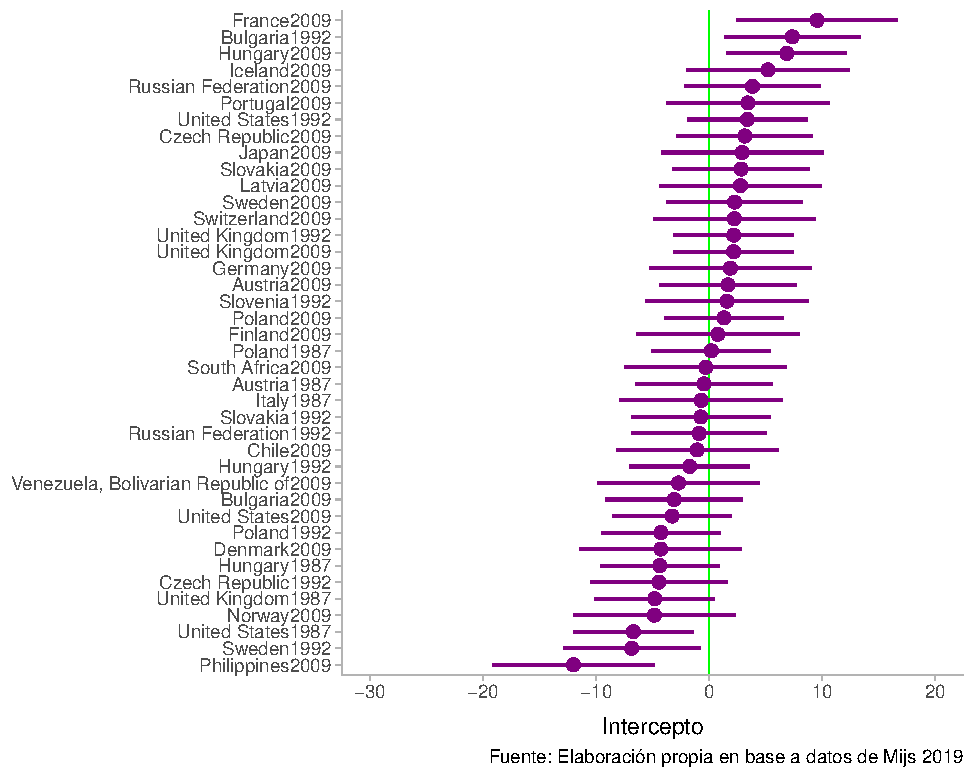
\includegraphics[width=1\linewidth]{03-guia_files/figure-latex/fig1-1} 

}

\caption{Interceptos aleatorios para Country-Wave del Modelo 1}\label{fig:fig1}
\end{figure}

En la Figura \ref{fig:fig2} se muestran los interceptos aleatorios del Modelo 1 a nivel de países (country). Similarmente a lo que ocurre a nivel de año-país, los resultados indican que, en su mayoría, los interceptos de los diferentes países no parecen desviarse significativamente de la gran media (\(\gamma_{000}\)). Unicamente Francia presenta valores superiores a la gran media que indican una mayor preocupación por la desigualdad (+7.68), mientras que Filipinas (-9.67) y Estados Unidos (-5.31) muestran valores menores a la gran media que se asocian con una preocupación significativamente menor por la desigualdad.

\begin{figure}

{\centering 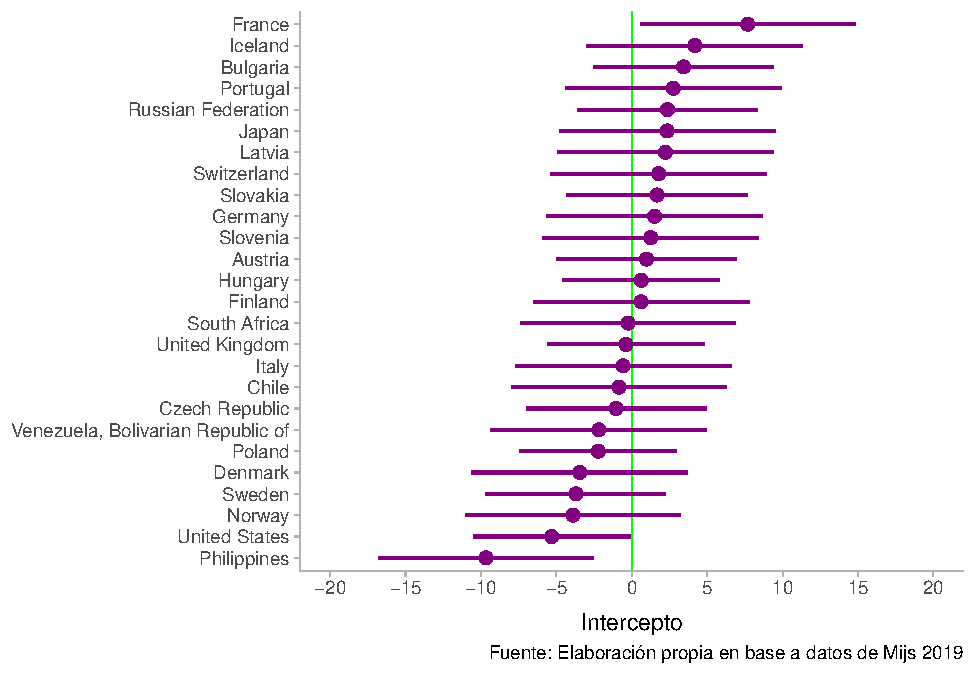
\includegraphics[width=1\linewidth]{03-guia_files/figure-latex/fig2-1} 

}

\caption{Interceptos aleatorios para Country del Modelo 1}\label{fig:fig2}
\end{figure}

\begin{enumerate}
\def\labelenumi{\alph{enumi})}
\setcounter{enumi}{3}
\tightlist
\item
  Interprete el efecto within de la percepción de desigualdad estructural sobre la preocupación por la misma (4 ptos).
\end{enumerate}

Los resultados del Modelo 1 (Tabla \ref{tab:table4}) sugieren que el efecto \emph{within} de la percepción de la desigualdad es positivo y estadísticamente significativo (\(\beta\) = 0.07, \(p\) \textless{} 0.001). Esto implica que, ceteris paribus, por cada unidad que un individuo aumenta en percepción de desigualdad respecto al promedio de su grupo (año-país), su preocupación por la desigualdad aumenta en 0.07 puntos en promedio. Dado que este predictor está centrado a la media grupal (CWC) a nivel de año-país (nivel 2), el coeficiente captura exclusivamente la variación dentro de cada año-país, eliminando la influencia de las diferencias promedio entre años-países o países (nivel 3). Esto significa que, para individuos dentro de un mismo año-país, aquellos que perciben una desigualdad mayor al promedio de su grupo también tienden a mostrar una mayor preocupación por la desigualdad.

\begin{enumerate}
\def\labelenumi{\alph{enumi})}
\setcounter{enumi}{4}
\tightlist
\item
  Compare e interprete los efectos between y contextual de la percepción de desigualdad a nivel 2, correspondientes a los modelos 1 y 2 (6 ptos).
\end{enumerate}

Los resultados del Modelo 1 (Tabla \ref{tab:table4}) sugieren que el efecto \emph{between-surveys} de la percepción de la desigualdad es positivo, pero no estadísticamente significativo (\(\beta\) = 0.66, \(p\) \textgreater{} 0.05). Este efecto refleja cómo las diferencias promedio en la percepción de la desigualdad a nivel de año-país están asociadas con la preocupación por la desigualdad a nivel individual. En detalle, esto indica que, controlando por las demás variables, por cada unidad de aumento en el promedio de percepción de desigualdad dentro de un año-país, la preocupación promedio por la desigualdad aumenta en 0.66 puntos a nivel individual. Sin embargo, esta relación no es estadísticamente significativa. Este predictor captura la variabilidad \emph{between-surveys}, es decir, las diferencias promedio en la percepción de desigualdad entre los diferentes años-países.

Por su parte, los resultados del Modelo 2 muestran que el efecto \emph{contextual-survey} de la percepción de desigualdad es positivo (\(\beta\) = 0.58) pero no estadísticamente significativo (\(p\) \textgreater{} 0.05). Este efecto representa la asociación entre el promedio de percepción de desigualdad a nivel de año-país (centrado a la gran media, CGM) y la preocupación individual por la desigualdad, controlando por la percepción de desigualdad a nivel individual. Es decir, ceteris paribus, un aumento de una unidad en el promedio de percepción de desigualdad a nivel de año-país/encuesta se asocia con un incremento promedio de 0.58 puntos en la escala de preocupación por la desigualdad, aunque esta relación no es estadísticamente significativa. Este efecto contextual captura cómo las diferencias en la percepción de desigualdad promedio entre años-países o encuestas están asociadas con la preocupación individual, considerando que las variaciones dentro de cada grupo están ya modeladas por el efecto \emph{within} Sin embargo, la falta de significancia estadística indica que esta relación no es robusta en este modelo.

Con todo, ninguno de los efectos \emph{between} o \emph{contextual} de la percepción de desigualdad a nivel de año-país/encuestas es estadísticamente significativo. Esto sugiere que las diferencias promedio en percepción de desigualdad entre años-países, ya sea como efecto \emph{between} o \emph{contextual}, no influyen de manera relevante en la preocupación individual por la desigualdad, controlando o no controlando por la percepción de desigualdad a nivel individual.

\begin{enumerate}
\def\labelenumi{\alph{enumi})}
\setcounter{enumi}{5}
\tightlist
\item
  Compare e interprete los efectos between y contextual de la percepción de desigualdad estructural a nivel 3, correspondientes a los modelos 1 y 2 (6 ptos).
\end{enumerate}

Los resultados del Modelo 1 (Tabla \ref{tab:table4}) sugieren que el efecto \emph{between-country} de la percepción de la desigualdad es positivo, pero no estadísticamente significativo (\(\beta\) = 0.51, \(p\) \textless{} 0.01). Este coeficiente indica que, en promedio, por cada unidad adicional en la percepción de desigualdad promedio de un país, la preocupación individual por la desigualdad aumenta en 0.51 puntos promedio. Este efecto captura exclusivamente las diferencias \emph{entre} países, sin controlar por variaciones dentro de los años-país o por predictores individuales. Por lo tanto, refleja cómo los contextos nacionales de percepción de desigualdad estructural están asociados con niveles más altos de preocupación por la desigualdad a nivel individual.

En cuanto al efecto \emph{contextual-country} de la percepción de desigualdad, los resultados del Modelo 2 sugieren que es negativo pero no estadísticamente significativo (\(\beta\) = -0.14, \(p\) \textgreater{} 0.05). Este efecto, representado por la media de percepción de desigualdad a nivel país (centrada a la gran media, CGM), captura cómo las diferencias promedio entre países influyen en la preocupación individual por la desigualdad, controlando por las variaciones dentro de los años-país y a nivel individual (ambas centradas CGM). Así, este coeficiente indica que, controlando por la percepción de desigualdad a nivel individual y año-país, un aumento de una unidad en el promedio de percepción de desigualdad de los países se asocia con una disminución de 0.14 puntos en la escala de preocupación por la desigualdad, aunque esta relación no es estadísticamente significativa.

Estos resultados permiten argumentar que las diferencias \emph{entre} países en la percepción de desigualdad (promedio) es relevante para explicar la preocupación por la desigualdad a nivel individual, sin controlar por variaciones a nivel año-país e individual. Sin embargo, el efecto \emph{contextual} de la percepción de desigualdad (promedio) de los países no es relevante para explicar la preocupación por la deisgualdad, ya que cuando se controla por el mismo predictor a nivel individual y de año-país, el efecto a nivel país no es estadísticamente significativo. Con todo, esto sugiere que las diferencias en la preocupación por la desigualdad se asocian en mayor medida a diferencias \emph{entre} países antes que a su efecto \emph{contextual}.

\hypertarget{enunciado-3}{%
\section{Enunciado 3}\label{enunciado-3}}

Estime un nuevo modelo (m3) utilizando la misma estructura de anidamiento. De la forma más parsimoniosa posible obtenga el efecto within de nivel 1 de la percepción de desigualdad, más las covariables mencionadas en la pregunta anterior. A continuación agregue los términos necesarios para obtener el efecto within-países y contextual-países del índice de Gini (Giniall).

\begin{enumerate}
\def\labelenumi{\alph{enumi})}
\tightlist
\item
  Reporte sus resultados en una tabla en formato académico (presente efectos al 90\%, 95\% y 99\% de confianza) (2 ptos)
\end{enumerate}

\begin{table}[H]
\begin{center}
\scalebox{0.8}{
\begin{threeparttable}
\begin{tabular}{l c}
\toprule
 & Modelo 3 \\
\midrule
Intercepto                                          & $78.71^{***}$ \\
                                                    & $(5.71)$      \\
Percepción de desigualdad (\textit{within})         & $0.07^{***}$  \\
                                                    & $(0.01)$      \\
Estudiante (\textit{CGM})                           & $-3.30^{***}$ \\
                                                    & $(0.78)$      \\
Edad (\textit{CGM})                                 & $0.04^{***}$  \\
                                                    & $(0.01)$      \\
Educación terciaria (\textit{CGM})                  & $-2.85^{***}$ \\
                                                    & $(0.27)$      \\
Mujer (\textit{CGM})                                & $2.44^{***}$  \\
                                                    & $(0.22)$      \\
Estatus social subjetivo (\textit{CGM})             & $-1.70^{***}$ \\
                                                    & $(0.07)$      \\
Desigualdad económica (\textit{within country})     & $0.70^{*}$    \\
                                                    & $(0.38)$      \\
Desigualdad económica (\textit{contextual country}) & $0.00$        \\
                                                    & $(0.17)$      \\
\midrule
AIC                                                 & $378667.92$   \\
BIC                                                 & $378771.59$   \\
Log Likelihood                                      & $-189321.96$  \\
Num. obs.                                           & $41739$       \\
Num. groups: country\_wave                          & $40$          \\
Num. groups: country                                & $26$          \\
Var: country\_wave (Intercept)                      & $23.63$       \\
Var: country (Intercept)                            & $42.84$       \\
Var: Residual                                       & $507.29$      \\
\bottomrule
\end{tabular}
\begin{tablenotes}[flushleft]
\scriptsize{\item Nota: Celdas contienen coeficientes de regresión con errores estándares entre paréntesis. $^{***}p<0.01$; $^{**}p<0.05$; $^{*}p<0.1$ \\ \item Fuente: Elaboración propia en base a datos de Mijs (2019)}
\end{tablenotes}
\end{threeparttable}
}
\caption{\label{tab:table5} Modelo multinivel para preocupación por la desigualdad según percepción de desigualdad, ser estudiante, edad, educación terciaria, sexo, estatus social subjetivo y desigualdad económica del país}
\label{table:coefficients}
\end{center}
\end{table}

\begin{enumerate}
\def\labelenumi{\alph{enumi})}
\setcounter{enumi}{1}
\tightlist
\item
  Compare e interprete sustantivamente los efectos within-países y contextual-países del índice de Gini y (10 ptos).
\end{enumerate}

En la Tabla \ref{tab:table5} se muestra el modelo multinivel estimado para predecir la preocupación por la desigualdad incorporando la desigualdad económica medida con el Índice de Gini. Los resultados de este modelo sugieren que el efecto \emph{within-country} de la desigualdad económica es positivo y estadísticamente significativo (\(\beta\) = 0.70, \(p\) \textless{} 0.1). En detalle, este coeficiente indica que, en promedio, un aumento de una unidad en la desigualdad económica de un mismo país en el tiempo (entre encuestas), se asocia con un incremento de 0.70 puntos en la escala de preocupación por la desigualdad, siendo esta relación estadísticamente significativa al 90\% de confianza. Este efecto captura las diferencias \emph{dentro} de los países en diferentes años-países o encuestas, cuando el promedio de la desigualdad económica aumenta en una unidad. Sustantivamente, este resultado sugiere que el aumento en el nivel de desigualdad económica \emph{dentro} de los países en el tiempo (encuestas/olas) influye positivamente en la preocupación por la desigualdad a nivel individual.

Por su parte, los resultados del Modelo 3 sugieren que el efecto \emph{contextual-country} de la desigualdad económica es positivo (casi nulo) pero no estadísticamente significativo (\(\beta\) = 0.00, \(p\) \textgreater{} 0.1). Especificamente, este coeficiente indica que por cada unidad adicional en el nivel de desigualdad en un país \emph{dentro} del mismo a lo largo del tiempo, la preocupación por la desigualdad aumenta en 0 puntos promedio, controlando por el nivel de desigualdad económica a nivel año-país. Sin embargo, este efecto no es estadísticamente significativo. Este predictor captura el efecto \emph{contextual} del país, ya que se encuentra controlado por el mismo predictor a nivel año-país o encuesta.

Los resultados apuntan a un hallazgo interesante: más que el efecto \emph{contextual} de la desigualdad económica del país, es su cambio \emph{dentro} de los países lo que explica en mayor medida la preocupación por la desigualdad a nivel individual. Dado que el efecto contextual de la desigualdad económica no es estadísticamente significativo, no es posible sostener que la ``tradición'' de desigualdad de un país tenga un impacto en la preocupación por la misma. Al contrario, el efecto \emph{within} países de la desigualdad económica sí se asocia con un incremento de la misma por parte de los individuos. Con todo, estos resultados resaltan la importancia de los cambios del nivel de desigualdad económica dentro de los países antes que su tendencia estructural para abordar la preocupación individual de la desigualdad.

\begin{enumerate}
\def\labelenumi{\alph{enumi})}
\setcounter{enumi}{2}
\tightlist
\item
  Estime un modelo (m4) que le permita evaluar la siguiente hipótesis: \emph{El efecto de la percepción de desigualdad sobre la preocupación por la misma, es moderada por el nivel objetivo de desigualdad del país en el largo plazo (promedio en el período)}. Reporte sus resultados y represéntelos gráficamente. Interprete sustantivamente (10 ptos).
\end{enumerate}

En la Tabla \ref{tab:table6} se muestra el modelo multinivel estimado para predecir la preocupación por la desigualdad incorporando la interacción entre la percepción de desigualdad y la desigualdad económica de los países. Los resultados sugieren que, cuando el nivel de desigualdad económica de los países \emph{(contextual-country)} aumenta en un porciento, el efecto \emph{within} de la percepción de la desigualdad es de 0,13 puntos promedios sobre la preocupación por la misma.

\begin{table}[H]
\begin{center}
\scalebox{0.8}{
\begin{threeparttable}
\begin{tabular}{l c}
\toprule
 & Modelo 4 \\
\midrule
Intercepto                                                                                        & $-498.68^{*}$ \\
                                                                                                  & $(274.18)$    \\
Percepción de desigualdad (\textit{within})                                                       & $0.14^{**}$   \\
                                                                                                  & $(0.06)$      \\
Estudiante (\textit{CGM})                                                                         & $-3.29^{***}$ \\
                                                                                                  & $(0.78)$      \\
Edad (\textit{CGM})                                                                               & $0.04^{***}$  \\
                                                                                                  & $(0.01)$      \\
Educación terciaria (\textit{CGM})                                                                & $-2.86^{***}$ \\
                                                                                                  & $(0.27)$      \\
Mujer (\textit{CGM})                                                                              & $2.45^{***}$  \\
                                                                                                  & $(0.22)$      \\
Estatus social subjetivo (\textit{CGM})                                                           & $-1.69^{***}$ \\
                                                                                                  & $(0.07)$      \\
Desigualdad económica (\textit{within country})                                                   & $-0.08$       \\
                                                                                                  & $(0.48)$      \\
Desigualdad económica (\textit{contextual country})                                               & $-0.04$       \\
                                                                                                  & $(0.37)$      \\
Percepción de desigualdad (\textit{within}) X Desigualdad económica (\textit{contextual country}) & $-0.00$       \\
                                                                                                  & $(0.00)$      \\
Ola                                                                                               & $0.29^{**}$   \\
                                                                                                  & $(0.14)$      \\
\midrule
AIC                                                                                               & $378624.22$   \\
BIC                                                                                               & $378762.45$   \\
Log Likelihood                                                                                    & $-189296.11$  \\
Num. obs.                                                                                         & $41739$       \\
Num. groups: country\_wave                                                                        & $40$          \\
Num. groups: country                                                                              & $26$          \\
Var: country\_wave (Intercept)                                                                    & $15.04$       \\
Var: country (Intercept)                                                                          & $296.40$      \\
Var: country inequality\_cgm1                                                                     & $0.01$        \\
Cov: country (Intercept) inequality\_cgm1                                                         & $0.50$        \\
Var: Residual                                                                                     & $505.56$      \\
\bottomrule
\end{tabular}
\begin{tablenotes}[flushleft]
\scriptsize{\item Nota: Celdas contienen coeficientes de regresión con errores estándares entre paréntesis. $^{***}p<0.01$; $^{**}p<0.05$; $^{*}p<0.1$ \\ \item Fuente: Elaboración propia en base a datos de Mijs (2019)}
\end{tablenotes}
\end{threeparttable}
}
\caption{\label{tab:table6} Modelo multinivel para preocupación por la desigualdad según percepción de desigualdad, desigualdad económica del periodo del país y covariables}
\label{table:coefficients}
\end{center}
\end{table}

En la Figura \ref{fig:fig3} se visualiza el efecto marginal de la percepción de desigualdad \emph{within}, moderada por el efecto \emph{contextual-country} del nivel de desigualdad económica. Los resultados indican que el efecto \emph{within} de la percepción de la desigualdad es positivo y estadísticamente significativo a medida que el nivel de desigualdad económica del país en el largo plazo o tradicionalmente oscila entre los valores 0 y 42. Sin embargo, a valores más extremos de desigualdad económica (superiores a 42 aprox.), el efecto \emph{within} de la percepción de la desigualdad deja de ser estadísticamente significativo. Sustantivamente, este resultado arroja hallazgos importantes, puesto que sugiere que la percepción de desigualdad a nivel individual afecta a la percepción de la misma cuando los países sostienen menores niveles de desigualdad económica en promedio. Por el otro lado, en países con mayores niveles de desigualdad, el efecto individual ``puro'' de la percepción subjetiva de la desigualdad no se asocia significativamente con la preocupación de la misma. Con todo, esto puede sugerir que el peso estructural de mayores niveles objetivo de desigualdad económica tiende a moderar o anular el efecto individual de la percepción subjetiva de la desigualdad, mientras que este efecto es mayor cuando la desigualdad económica de los países es menor.

\begin{figure}

{\centering 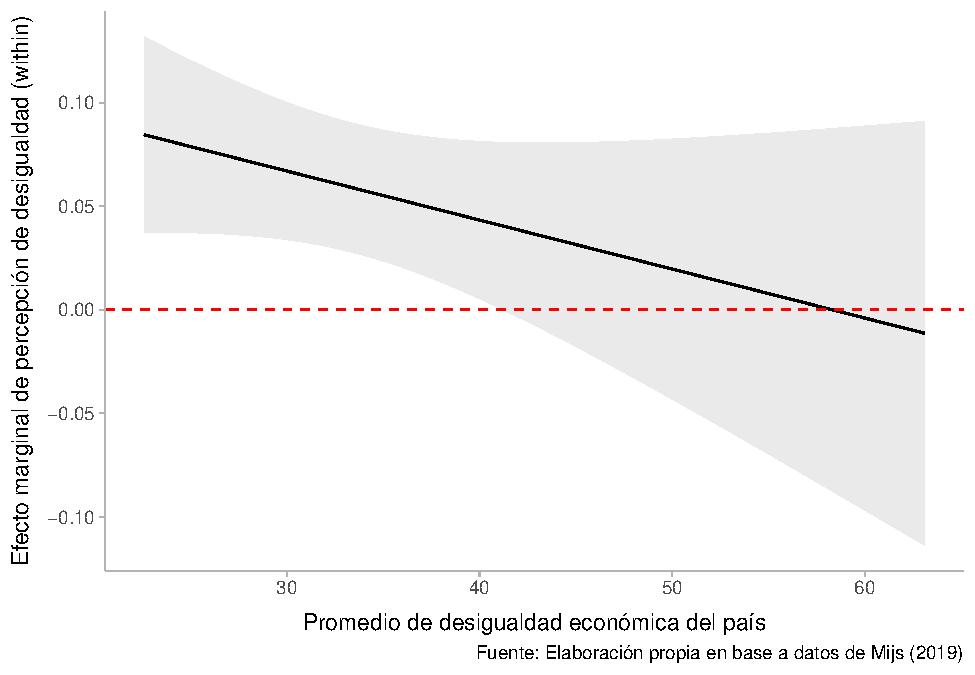
\includegraphics[width=0.8\linewidth]{03-guia_files/figure-latex/fig3-1} 

}

\caption{Efecto marginal del efecto within de percepción de desigualdad moderado por el efecto contextual de desigualdad económica del país}\label{fig:fig3}
\end{figure}

\begin{enumerate}
\def\labelenumi{\alph{enumi})}
\setcounter{enumi}{3}
\tightlist
\item
  Tomando como referencia el modelo 3 evalúe si existen observaciones influyentes. Reporte sus análisis y concluya (8 ptos).
\end{enumerate}

En la Figura \ref{fig:fig4} se muestra la distancia de Cook para observaciones influyentes en el Modelo 3. Se optó por utilizar la prueba de distancia de Cook con el fin de obtener una evaluación general que resume la influencia de las observaciones (países) sobre el total de parámetros en el modelo. El punto de corte es 0.1538462, considerando que existen 26 países en la base de datos.

Los resultados sugieren que existe una buena cantidad de países que apalancan el Modelo 3. En total, los países que pasan el punto de corte (marcados por triangulos rojos), alcazan los 12 de un total de 26, es decir, casi la mitad de los países. El país que más se aleja del punto de corte es Dinamarca, seguido por Sudafrica y Suecia.

\begin{figure}

{\centering 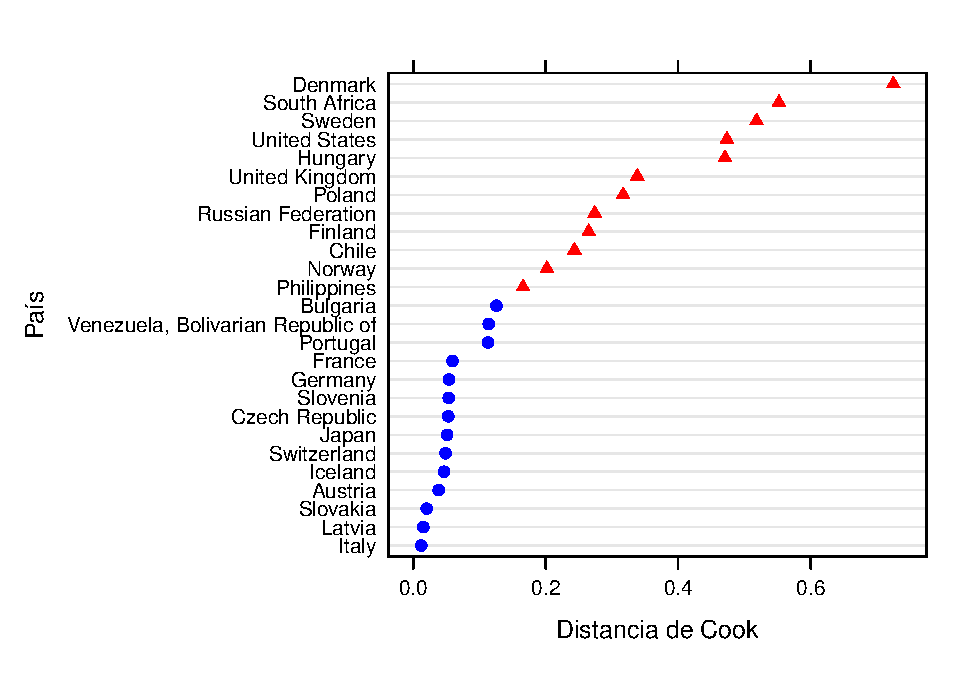
\includegraphics[width=0.9\linewidth]{03-guia_files/figure-latex/fig4-1} 

}

\caption{Distancia de Cook para observaciones influyentes en el Modelo 3}\label{fig:fig4}
\end{figure}

Para determinar si la exclusión de alguna de estas observaciones influyentes afectan la signifancia estadística de los parámetros fijos estimados en el Modelo 3, se condujo una prueba de cambios de significancia estadística (ver Tabla \ref{tab:table7}). De acuerdo con los resultados de esta prueba, no existe evidencia que los países cambien la significancia estadística de los parámetros estimados en el Modelo 3. En definitiva, estos resultados permiten sostener que no es necesario remover ningún país y que las estimaciones del Modelo 3 se mantienen robustas.

\begin{table}[H]

\caption{\label{tab:table7}\label{tab:table7} Estadísticos de cambio de significancia estadística para el Modelo 3}
\centering
\fontsize{10}{12}\selectfont
\begin{tabu} to \linewidth {>{\raggedright\arraybackslash}p{2cm}>{\raggedright}X>{\raggedright}X>{\raggedright}X>{\raggedright}X>{\raggedright}X>{\raggedright}X>{\raggedright}X>{\raggedright}X>{\raggedright}X}
\toprule
\textbf{País} & \textbf{Intercepto} & \textbf{Percepción desigualdad (within)} & \textbf{Estudiante (cgm)} & \textbf{Edad (cgm)} & \textbf{Educ. Terciaria (cgm)} & \textbf{Mujer (cgm)} & \textbf{ESS (cgm)} & \textbf{Gini (within-country)} & \textbf{Gini (contextual-country)}\\
\midrule
Austria & FALSE & FALSE & FALSE & FALSE & FALSE & FALSE & FALSE & FALSE & FALSE\\
Bulgaria & FALSE & FALSE & FALSE & FALSE & FALSE & FALSE & FALSE & FALSE & FALSE\\
Chile & FALSE & FALSE & FALSE & FALSE & FALSE & FALSE & FALSE & FALSE & FALSE\\
Czech Republic & FALSE & FALSE & FALSE & FALSE & FALSE & FALSE & FALSE & FALSE & FALSE\\
Denmark & FALSE & FALSE & FALSE & FALSE & FALSE & FALSE & FALSE & FALSE & FALSE\\
\addlinespace
Finland & FALSE & FALSE & FALSE & FALSE & FALSE & FALSE & FALSE & FALSE & FALSE\\
France & FALSE & FALSE & FALSE & FALSE & FALSE & FALSE & FALSE & FALSE & FALSE\\
Germany & FALSE & FALSE & FALSE & FALSE & FALSE & FALSE & FALSE & FALSE & FALSE\\
Hungary & FALSE & FALSE & FALSE & FALSE & FALSE & FALSE & FALSE & FALSE & FALSE\\
Iceland & FALSE & FALSE & FALSE & FALSE & FALSE & FALSE & FALSE & FALSE & FALSE\\
\addlinespace
Italy & FALSE & FALSE & FALSE & FALSE & FALSE & FALSE & FALSE & FALSE & FALSE\\
Japan & FALSE & FALSE & FALSE & FALSE & FALSE & FALSE & FALSE & FALSE & FALSE\\
Latvia & FALSE & FALSE & FALSE & FALSE & FALSE & FALSE & FALSE & FALSE & FALSE\\
Norway & FALSE & FALSE & FALSE & FALSE & FALSE & FALSE & FALSE & FALSE & FALSE\\
Philippines & FALSE & FALSE & FALSE & FALSE & FALSE & FALSE & FALSE & FALSE & FALSE\\
\addlinespace
Poland & FALSE & FALSE & FALSE & FALSE & FALSE & FALSE & FALSE & FALSE & FALSE\\
Portugal & FALSE & FALSE & FALSE & FALSE & FALSE & FALSE & FALSE & FALSE & FALSE\\
Russian Federation & FALSE & FALSE & FALSE & FALSE & FALSE & FALSE & FALSE & FALSE & FALSE\\
Slovakia & FALSE & FALSE & FALSE & FALSE & FALSE & FALSE & FALSE & FALSE & FALSE\\
Slovenia & FALSE & FALSE & FALSE & FALSE & FALSE & FALSE & FALSE & FALSE & FALSE\\
\addlinespace
South Africa & FALSE & FALSE & FALSE & FALSE & FALSE & FALSE & FALSE & FALSE & FALSE\\
Sweden & FALSE & FALSE & FALSE & FALSE & FALSE & FALSE & FALSE & FALSE & FALSE\\
Switzerland & FALSE & FALSE & FALSE & FALSE & FALSE & FALSE & FALSE & FALSE & FALSE\\
United Kingdom & FALSE & FALSE & FALSE & FALSE & FALSE & FALSE & FALSE & FALSE & FALSE\\
United States & FALSE & FALSE & FALSE & FALSE & FALSE & FALSE & FALSE & FALSE & FALSE\\
\addlinespace
Venezuela, Bolivarian Republic of & FALSE & FALSE & FALSE & FALSE & FALSE & FALSE & FALSE & FALSE & FALSE\\
\bottomrule
\multicolumn{10}{l}{\textsuperscript{} Fuente: Elaboración propia en base a datos de Mijs (2019).}\\
\end{tabu}
\end{table}

\pagebreak

\hypertarget{referencias}{%
\section{Referencias}\label{referencias}}

\hypertarget{refs}{}
\begin{CSLReferences}{1}{0}
\leavevmode\vadjust pre{\hypertarget{ref-fairbrotherTwoMultilevelModeling2014}{}}%
Fairbrother, M. (2014). Two {Multilevel Modeling Techniques} for {Analyzing Comparative Longitudinal Survey Datasets}. \emph{Political Science Research and Methods}, \emph{2}(1), 119--140. \url{https://doi.org/10.1017/psrm.2013.24}

\leavevmode\vadjust pre{\hypertarget{ref-schmidt-catranRandomEffectsMultilevel2016}{}}%
Schmidt-Catran, A. W., \& Fairbrother, M. (2016). The {Random Effects} in {Multilevel Models}: {Getting Them Wrong} and {Getting Them Right}. \emph{European Sociological Review}, \emph{32}(1), 23--38. \url{https://doi.org/10.1093/esr/jcv090}

\end{CSLReferences}

\pagebreak

\hypertarget{cuxf3digo-de-r}{%
\section{Código de R}\label{cuxf3digo-de-r}}

\begin{Shaded}
\begin{Highlighting}[]
\NormalTok{knitr}\SpecialCharTok{::}\NormalTok{opts\_chunk}\SpecialCharTok{$}\FunctionTok{set}\NormalTok{(}\AttributeTok{echo =}\NormalTok{ F,}
                      \AttributeTok{warning =}\NormalTok{ F,}
                      \AttributeTok{error =}\NormalTok{ F, }
                      \AttributeTok{message =}\NormalTok{ F) }
\ControlFlowTok{if}\NormalTok{ (}\SpecialCharTok{!} \FunctionTok{require}\NormalTok{(}\StringTok{"pacman"}\NormalTok{)) }\FunctionTok{install.packages}\NormalTok{(}\StringTok{"pacman"}\NormalTok{)}

\NormalTok{pacman}\SpecialCharTok{::}\FunctionTok{p\_load}\NormalTok{(tidyverse, }
\NormalTok{               magrittr,}
\NormalTok{               sjmisc, }
\NormalTok{               sjPlot, }
\NormalTok{               lme4, }
\NormalTok{               easystats, }
\NormalTok{               influence.ME, }
\NormalTok{               broom.mixed, }
\NormalTok{               here,}
\NormalTok{               marginaleffects,}
\NormalTok{               ggeffects,}
\NormalTok{               texreg, }
\NormalTok{               ggdist,}
\NormalTok{               misty,}
\NormalTok{               kableExtra,}
\NormalTok{               cowplot,}
\NormalTok{               patchwork)}

\FunctionTok{options}\NormalTok{(}\AttributeTok{scipen=}\DecValTok{999}\NormalTok{)}
\FunctionTok{rm}\NormalTok{(}\AttributeTok{list =} \FunctionTok{ls}\NormalTok{())}

\NormalTok{miles }\OtherTok{\textless{}{-}} \ControlFlowTok{function}\NormalTok{(x) \{}
  \FunctionTok{format}\NormalTok{(}\FunctionTok{round}\NormalTok{(}\FunctionTok{as.numeric}\NormalTok{(x),}\DecValTok{0}\NormalTok{), }\AttributeTok{big.mark =} \StringTok{"."}\NormalTok{)}
\NormalTok{\}}

\NormalTok{decimales }\OtherTok{\textless{}{-}} \ControlFlowTok{function}\NormalTok{(x) \{}
  \FunctionTok{format}\NormalTok{(}\FunctionTok{round}\NormalTok{(}\FunctionTok{as.numeric}\NormalTok{(x), }\DecValTok{2}\NormalTok{), }\AttributeTok{decimal.mark =} \StringTok{","}\NormalTok{)}
\NormalTok{\}}

\CommentTok{\# set theme}

\FunctionTok{theme\_set}\NormalTok{(}\FunctionTok{theme\_ggdist}\NormalTok{())}

\FunctionTok{options}\NormalTok{(}\AttributeTok{knitr.kable.NA =} \StringTok{""}\NormalTok{)}
\FunctionTok{options}\NormalTok{(}\AttributeTok{knitr.table.format=}\StringTok{"latex"}\NormalTok{)}

\FunctionTok{load}\NormalTok{(}\AttributeTok{file =} \FunctionTok{here}\NormalTok{(}\StringTok{"input/data/issp\_merge.RData"}\NormalTok{)) }\SpecialCharTok{\%\textgreater{}\%} 
\NormalTok{  sjlabelled}\SpecialCharTok{::}\FunctionTok{remove\_all\_labels}\NormalTok{()}

\FunctionTok{names}\NormalTok{(issp\_merge)}
\FunctionTok{glimpse}\NormalTok{(issp\_merge)}

\CommentTok{\# seleccionar {-}{-}{-}{-}}

\NormalTok{db }\OtherTok{\textless{}{-}}\NormalTok{ issp\_merge }\SpecialCharTok{\%\textgreater{}\%} 
\NormalTok{  dplyr}\SpecialCharTok{::}\FunctionTok{select}\NormalTok{(caseid, countryR, year, ID.issp, region, concern, merit, inequality, employed, student, retired, age, socestat, educ.prim, educ.second, educ.terc, female, Giniall) }\SpecialCharTok{\%\textgreater{}\%} 
\NormalTok{  janitor}\SpecialCharTok{::}\FunctionTok{clean\_names}\NormalTok{() }\SpecialCharTok{\%\textgreater{}\%} 
  \FunctionTok{as\_tibble}\NormalTok{() }\SpecialCharTok{\%\textgreater{}\%} 
\NormalTok{  sjlabelled}\SpecialCharTok{::}\FunctionTok{remove\_all\_labels}\NormalTok{()}
 
\CommentTok{\# filtrar: no {-}{-}{-}{-}{-} }

\CommentTok{\# recodificar y transformar: luego {-}{-}{-}{-}}

\NormalTok{db }\SpecialCharTok{\%\textgreater{}\%} 
  \FunctionTok{select}\NormalTok{(concern, inequality, merit) }\SpecialCharTok{\%\textgreater{}\%}
\NormalTok{  sjmisc}\SpecialCharTok{::}\FunctionTok{descr}\NormalTok{(.)}

\NormalTok{db}\SpecialCharTok{$}\NormalTok{year }\OtherTok{\textless{}{-}} \FunctionTok{as.numeric}\NormalTok{(db}\SpecialCharTok{$}\NormalTok{year)}

\NormalTok{db }\OtherTok{\textless{}{-}}\NormalTok{ db }\SpecialCharTok{\%\textgreater{}\%} 
  \FunctionTok{rename}\NormalTok{(}\AttributeTok{country\_wave =}\NormalTok{ id\_issp,}
         \AttributeTok{country =}\NormalTok{ country\_r,}
         \AttributeTok{wave =}\NormalTok{ year)}

\CommentTok{\# casos perdidos {-}{-}{-}{-}{-}}

\FunctionTok{colSums}\NormalTok{(}\FunctionTok{is.na}\NormalTok{(db))}

\CommentTok{\#db \textless{}{-} na.omit(db)}


\NormalTok{mA }\OtherTok{\textless{}{-}} \FunctionTok{lmer}\NormalTok{(concern }\SpecialCharTok{\textasciitilde{}} \DecValTok{1} \SpecialCharTok{+}\NormalTok{ (}\DecValTok{1} \SpecialCharTok{|}\NormalTok{ country\_wave), }\AttributeTok{data =}\NormalTok{ db)}
\NormalTok{mB }\OtherTok{\textless{}{-}} \FunctionTok{lmer}\NormalTok{(concern }\SpecialCharTok{\textasciitilde{}} \DecValTok{1} \SpecialCharTok{+}\NormalTok{ (}\DecValTok{1} \SpecialCharTok{|}\NormalTok{ country), }\AttributeTok{data =}\NormalTok{ db)}
\NormalTok{mC }\OtherTok{\textless{}{-}} \FunctionTok{lmer}\NormalTok{(concern }\SpecialCharTok{\textasciitilde{}} \DecValTok{1} \SpecialCharTok{+}\NormalTok{ (}\DecValTok{1} \SpecialCharTok{|}\NormalTok{ country\_wave) }\SpecialCharTok{+}\NormalTok{ (}\DecValTok{1} \SpecialCharTok{|}\NormalTok{ wave), }\AttributeTok{data =}\NormalTok{ db)}
\NormalTok{mD }\OtherTok{\textless{}{-}} \FunctionTok{lmer}\NormalTok{(concern }\SpecialCharTok{\textasciitilde{}} \DecValTok{1} \SpecialCharTok{+}\NormalTok{ (}\DecValTok{1} \SpecialCharTok{|}\NormalTok{ country\_wave) }\SpecialCharTok{+}\NormalTok{ (}\DecValTok{1} \SpecialCharTok{|}\NormalTok{ country), }\AttributeTok{data =}\NormalTok{ db)}
\NormalTok{mE }\OtherTok{\textless{}{-}} \FunctionTok{lmer}\NormalTok{(concern }\SpecialCharTok{\textasciitilde{}} \DecValTok{1} \SpecialCharTok{+}\NormalTok{ (}\DecValTok{1} \SpecialCharTok{|}\NormalTok{ country) }\SpecialCharTok{+}\NormalTok{ (}\DecValTok{1} \SpecialCharTok{|}\NormalTok{ wave), }\AttributeTok{data =}\NormalTok{ db)}
\NormalTok{mF }\OtherTok{\textless{}{-}} \FunctionTok{lmer}\NormalTok{(concern }\SpecialCharTok{\textasciitilde{}} \DecValTok{1} \SpecialCharTok{+}\NormalTok{ (}\DecValTok{1} \SpecialCharTok{|}\NormalTok{ country\_wave) }\SpecialCharTok{+}\NormalTok{ (}\DecValTok{1} \SpecialCharTok{|}\NormalTok{ country) }\SpecialCharTok{+}
\NormalTok{             (}\DecValTok{1} \SpecialCharTok{|}\NormalTok{ wave), }\AttributeTok{data =}\NormalTok{ db) }


\NormalTok{ccoef }\OtherTok{\textless{}{-}} \FunctionTok{list}\NormalTok{(}
  \StringTok{"(Intercept)"} \OtherTok{=} \StringTok{"Intercepto"}\NormalTok{)}

\NormalTok{texreg}\SpecialCharTok{::}\FunctionTok{texreg}\NormalTok{(}\FunctionTok{list}\NormalTok{(mA,mB,mC,mD,mE,mF),}
               \AttributeTok{custom.model.names =} \FunctionTok{c}\NormalTok{(}\StringTok{"Modelo (A)"}\NormalTok{,}
                                      \StringTok{"Modelo (B)"}\NormalTok{,}
                                      \StringTok{"Modelo (C)"}\NormalTok{,}
                                      \StringTok{"Modelo (D)"}\NormalTok{,}
                                      \StringTok{"Modelo (E)"}\NormalTok{,}
                                      \StringTok{"Modelo (F)"}\NormalTok{),}
               \AttributeTok{caption =} \FunctionTok{paste}\NormalTok{(}\StringTok{"(}\SpecialCharTok{\textbackslash{}\textbackslash{}}\StringTok{\#tab:table1)"}\NormalTok{,}\StringTok{"Modelos multinivel nulos para preocupación por la desigualdad con diferentes estructuras de efectos aleatorios"}\NormalTok{),}
               \AttributeTok{stars =} \FunctionTok{c}\NormalTok{(}\FloatTok{0.05}\NormalTok{, }\FloatTok{0.01}\NormalTok{, }\FloatTok{0.001}\NormalTok{),}
               \AttributeTok{custom.coef.map =}\NormalTok{ ccoef,}
               \AttributeTok{custom.note =} \StringTok{"}\SpecialCharTok{\textbackslash{}\textbackslash{}}\StringTok{item Nota: Celdas contienen coeficientes de regresión con errores estándares entre paréntesis. \%stars. Modelo (A) = Country{-}Year, Modelo (B) = Country, Modelo (C) = Year/Country{-}Year, Modelo (D) = Country/Country{-}Year, Modelo (E) = Country/Year, Modelo (F) = Country/Year/Country{-}Year }\SpecialCharTok{\textbackslash{}\textbackslash{}\textbackslash{}\textbackslash{}}\StringTok{ }\SpecialCharTok{\textbackslash{}\textbackslash{}}\StringTok{item Fuente: Elaboración propia en base a datos de Mijs (2019)."}\NormalTok{,}
               \AttributeTok{threeparttable =}\NormalTok{ T,}
               \AttributeTok{leading.zero =}\NormalTok{ T,}
               \AttributeTok{float.pos =} \StringTok{"h!"}\NormalTok{,}
               \AttributeTok{use.packages =}\NormalTok{ F,}
               \AttributeTok{booktabs =}\NormalTok{ T,}
               \AttributeTok{scalebox =} \FloatTok{0.8}\NormalTok{)}

\NormalTok{tab\_icc }\OtherTok{\textless{}{-}} \FunctionTok{bind\_rows}\NormalTok{(                                                 }
\NormalTok{performance}\SpecialCharTok{::}\FunctionTok{icc}\NormalTok{(mA, }\AttributeTok{by\_group =}\NormalTok{ T) }\SpecialCharTok{\%\textgreater{}\%} 
  \FunctionTok{as\_tibble}\NormalTok{() }\SpecialCharTok{\%\textgreater{}\%} 
  \FunctionTok{mutate}\NormalTok{(}\AttributeTok{Model =} \StringTok{"Modelo (A) Country{-}Year"}\NormalTok{),}
\NormalTok{performance}\SpecialCharTok{::}\FunctionTok{icc}\NormalTok{(mB, }\AttributeTok{by\_group =}\NormalTok{ T) }\SpecialCharTok{\%\textgreater{}\%} 
  \FunctionTok{as\_tibble}\NormalTok{() }\SpecialCharTok{\%\textgreater{}\%} 
  \FunctionTok{mutate}\NormalTok{(}\AttributeTok{Model =}  \StringTok{"Modelo (B) Country"}\NormalTok{),}
\NormalTok{performance}\SpecialCharTok{::}\FunctionTok{icc}\NormalTok{(mC, }\AttributeTok{by\_group =}\NormalTok{ T) }\SpecialCharTok{\%\textgreater{}\%} 
  \FunctionTok{as\_tibble}\NormalTok{() }\SpecialCharTok{\%\textgreater{}\%} 
  \FunctionTok{mutate}\NormalTok{(}\AttributeTok{Model =} \StringTok{"Modelo (C) Year/Country{-}Year"}\NormalTok{),}
\NormalTok{performance}\SpecialCharTok{::}\FunctionTok{icc}\NormalTok{(mD, }\AttributeTok{by\_group =}\NormalTok{ T) }\SpecialCharTok{\%\textgreater{}\%} 
  \FunctionTok{as\_tibble}\NormalTok{() }\SpecialCharTok{\%\textgreater{}\%} 
  \FunctionTok{mutate}\NormalTok{(}\AttributeTok{Model =} \StringTok{"Modelo (D) Country/Country{-}Year"}\NormalTok{),}
\NormalTok{performance}\SpecialCharTok{::}\FunctionTok{icc}\NormalTok{(mE, }\AttributeTok{by\_group =}\NormalTok{ T) }\SpecialCharTok{\%\textgreater{}\%} 
  \FunctionTok{as\_tibble}\NormalTok{() }\SpecialCharTok{\%\textgreater{}\%} 
  \FunctionTok{mutate}\NormalTok{(}\AttributeTok{Model =} \StringTok{"Modelo (E) Country/Year"}\NormalTok{),}
\NormalTok{performance}\SpecialCharTok{::}\FunctionTok{icc}\NormalTok{(mF, }\AttributeTok{by\_group =}\NormalTok{ T) }\SpecialCharTok{\%\textgreater{}\%} 
  \FunctionTok{as\_tibble}\NormalTok{() }\SpecialCharTok{\%\textgreater{}\%} 
  \FunctionTok{mutate}\NormalTok{(}\AttributeTok{Model =} \StringTok{"Modelo (F) Country/Year/Country{-}Year"}\NormalTok{),}
\NormalTok{) }\SpecialCharTok{\%\textgreater{}\%} 
  \FunctionTok{select}\NormalTok{(Model, Group, ICC) }\SpecialCharTok{\%\textgreater{}\%} 
  \FunctionTok{mutate}\NormalTok{(}\AttributeTok{ICC =} \FunctionTok{round}\NormalTok{(ICC, }\DecValTok{3}\NormalTok{)) }

\NormalTok{tab\_icc }\SpecialCharTok{\%\textgreater{}\%} 
  \FunctionTok{filter}\NormalTok{(}\FunctionTok{str\_detect}\NormalTok{(Model, }\StringTok{"D|F"}\NormalTok{)) }\SpecialCharTok{\%\textgreater{}\%} 
\NormalTok{  kableExtra}\SpecialCharTok{::}\FunctionTok{kable}\NormalTok{(}\AttributeTok{format =} \StringTok{"latex"}\NormalTok{, }
                    \AttributeTok{col.names =} \FunctionTok{c}\NormalTok{(}\StringTok{"Modelo"}\NormalTok{, }\StringTok{"Unidad"}\NormalTok{, }\StringTok{"ICC"}\NormalTok{),}
                    \AttributeTok{row.names =}\NormalTok{ F,}
                    \AttributeTok{booktabs =}\NormalTok{ T, }\AttributeTok{align =} \StringTok{\textquotesingle{}l\textquotesingle{}}\NormalTok{,}
                    \AttributeTok{caption =} \FunctionTok{paste}\NormalTok{(}\StringTok{"(}\SpecialCharTok{\textbackslash{}\textbackslash{}}\StringTok{\#tab:table2)"}\NormalTok{,}\StringTok{"Comparación de correlación intraclase para preocupación por la desigualdad entre diferentes estructuras de efectos aleatorios"}\NormalTok{)) }\SpecialCharTok{\%\textgreater{}\%} 
\NormalTok{  kableExtra}\SpecialCharTok{::}\FunctionTok{kable\_styling}\NormalTok{(}\AttributeTok{latex\_options =} \StringTok{"hold\_position"}\NormalTok{, }
                            \AttributeTok{position =} \StringTok{"center"}\NormalTok{) }\SpecialCharTok{\%\textgreater{}\%}
\NormalTok{  kableExtra}\SpecialCharTok{::}\FunctionTok{kable\_styling}\NormalTok{(}\AttributeTok{bootstrap\_options =} \FunctionTok{c}\NormalTok{(}\StringTok{"striped"}\NormalTok{, }\StringTok{"hover"}\NormalTok{, }\StringTok{"condensed"}\NormalTok{, }\StringTok{"responsive"}\NormalTok{), }\AttributeTok{full\_width =}\NormalTok{ F) }\SpecialCharTok{\%\textgreater{}\%} 
\NormalTok{  kableExtra}\SpecialCharTok{::}\FunctionTok{column\_spec}\NormalTok{(}\DecValTok{1}\NormalTok{, }\AttributeTok{width =} \StringTok{"8cm"}\NormalTok{) }\SpecialCharTok{\%\textgreater{}\%}
\NormalTok{  kableExtra}\SpecialCharTok{::}\FunctionTok{row\_spec}\NormalTok{(}\DecValTok{0}\NormalTok{, }\AttributeTok{bold =}\NormalTok{ T) }\SpecialCharTok{\%\textgreater{}\%} 
\NormalTok{  kableExtra}\SpecialCharTok{::}\FunctionTok{add\_footnote}\NormalTok{(}\AttributeTok{label =} \StringTok{"Fuente: Elaboración propia en base a datos de Mijs (2019)."}\NormalTok{, }\AttributeTok{notation =} \StringTok{"none"}\NormalTok{)}
  
 


\NormalTok{res\_fit1 }\OtherTok{\textless{}{-}} \FunctionTok{anova}\NormalTok{(mF, mD)}

\NormalTok{fit\_tab }\OtherTok{\textless{}{-}}\NormalTok{ res\_fit1[}\FunctionTok{c}\NormalTok{(}\DecValTok{2}\NormalTok{,}\DecValTok{3}\NormalTok{,}\DecValTok{5}\NormalTok{,}\DecValTok{6}\NormalTok{,}\DecValTok{7}\NormalTok{,}\DecValTok{8}\NormalTok{)] }\SpecialCharTok{\%\textgreater{}\%} \FunctionTok{as\_tibble}\NormalTok{(.)}

\NormalTok{fit\_tab}\SpecialCharTok{$}\NormalTok{mod }\OtherTok{\textless{}{-}} \FunctionTok{c}\NormalTok{(}\StringTok{"Modelo D"}\NormalTok{, }\StringTok{"Modelo F"}\NormalTok{)}

\NormalTok{fit\_tab}\SpecialCharTok{$}\NormalTok{p }\OtherTok{\textless{}{-}} \FunctionTok{if\_else}\NormalTok{(fit\_tab}\SpecialCharTok{$}\StringTok{\textasciigrave{}}\AttributeTok{Pr(\textgreater{}Chisq)}\StringTok{\textasciigrave{}} \SpecialCharTok{\textless{}} \FloatTok{0.05}\NormalTok{, }\StringTok{"p \textless{} 0.05 *"}\NormalTok{, }\StringTok{"p \textgreater{} 0.05"}\NormalTok{)}

\NormalTok{fit\_tab}\SpecialCharTok{$}\NormalTok{Chisq }\OtherTok{\textless{}{-}} \FunctionTok{round}\NormalTok{(fit\_tab}\SpecialCharTok{$}\NormalTok{Chisq, }\AttributeTok{digits =} \DecValTok{2}\NormalTok{)}

\NormalTok{fit\_tab }\OtherTok{\textless{}{-}}\NormalTok{ fit\_tab }\SpecialCharTok{\%\textgreater{}\%} 
\NormalTok{  dplyr}\SpecialCharTok{::}\FunctionTok{select}\NormalTok{(mod, AIC, BIC, deviance, Chisq, Df, p)}

\NormalTok{colnames }\OtherTok{\textless{}{-}} \FunctionTok{c}\NormalTok{(}\StringTok{"Modelo"}\NormalTok{, }\StringTok{"AIC"}\NormalTok{, }\StringTok{"BIC"}\NormalTok{, }\StringTok{"Deviance"}\NormalTok{, }\StringTok{"X2"}\NormalTok{, }\StringTok{"Df"}\NormalTok{, }\StringTok{"p{-}value"}\NormalTok{)}

\NormalTok{fit\_tab }\OtherTok{\textless{}{-}}\NormalTok{ kableExtra}\SpecialCharTok{::}\FunctionTok{kable}\NormalTok{(fit\_tab, }
                             \AttributeTok{format =} \StringTok{"latex"}\NormalTok{, }
                             \AttributeTok{col.names =}\NormalTok{ colnames,}
                             \AttributeTok{row.names =}\NormalTok{ F,}
                             \AttributeTok{booktabs =}\NormalTok{ T, }
                             \AttributeTok{caption =} \FunctionTok{paste}\NormalTok{(}\StringTok{"(}\SpecialCharTok{\textbackslash{}\textbackslash{}}\StringTok{\#tab:table3)"}\NormalTok{,}\StringTok{"Estadísticos de bondad de ajuste entre Modelo D y Modelo F"}\NormalTok{)) }\SpecialCharTok{\%\textgreater{}\%} 
\NormalTok{  kableExtra}\SpecialCharTok{::}\FunctionTok{kable\_styling}\NormalTok{(}\AttributeTok{latex\_options =} \StringTok{"hold\_position"}\NormalTok{, }
                            \AttributeTok{position =} \StringTok{"center"}\NormalTok{) }\SpecialCharTok{\%\textgreater{}\%}
\NormalTok{  kableExtra}\SpecialCharTok{::}\FunctionTok{kable\_styling}\NormalTok{(}\AttributeTok{bootstrap\_options =} \FunctionTok{c}\NormalTok{(}\StringTok{"striped"}\NormalTok{, }\StringTok{"hover"}\NormalTok{, }\StringTok{"condensed"}\NormalTok{, }\StringTok{"responsive"}\NormalTok{), }\AttributeTok{full\_width =}\NormalTok{ F) }\SpecialCharTok{\%\textgreater{}\%} 
\NormalTok{  kableExtra}\SpecialCharTok{::}\FunctionTok{column\_spec}\NormalTok{(}\DecValTok{1}\NormalTok{, }\AttributeTok{width =} \StringTok{"2cm"}\NormalTok{) }\SpecialCharTok{\%\textgreater{}\%}
\NormalTok{  kableExtra}\SpecialCharTok{::}\FunctionTok{row\_spec}\NormalTok{(}\DecValTok{0}\NormalTok{, }\AttributeTok{bold =}\NormalTok{ T) }\SpecialCharTok{\%\textgreater{}\%} 
\NormalTok{  kableExtra}\SpecialCharTok{::}\FunctionTok{add\_footnote}\NormalTok{(}\AttributeTok{label =} \FunctionTok{c}\NormalTok{(}\StringTok{"Fuente: Elaboración propia en base a datos de Mijs (2019)."}\NormalTok{), }\AttributeTok{notation =} \StringTok{"none"}\NormalTok{)}

\NormalTok{fit\_tab}

\NormalTok{db }\SpecialCharTok{\%\textless{}\textgreater{}\%} 
  \FunctionTok{group\_by}\NormalTok{(country\_wave) }\SpecialCharTok{\%\textgreater{}\%}
  \FunctionTok{mutate}\NormalTok{(}\AttributeTok{cm\_inequality\_country\_wave =} \FunctionTok{mean}\NormalTok{(inequality, }\AttributeTok{na.rm =}\NormalTok{ T)) }\SpecialCharTok{\%\textgreater{}\%} 
  \FunctionTok{ungroup}\NormalTok{() }

\NormalTok{db }\SpecialCharTok{\%\textless{}\textgreater{}\%} 
  \FunctionTok{group\_by}\NormalTok{(country) }\SpecialCharTok{\%\textgreater{}\%}
  \FunctionTok{mutate}\NormalTok{(}\AttributeTok{cm\_inequality\_country =} \FunctionTok{mean}\NormalTok{(inequality, }\AttributeTok{na.rm =}\NormalTok{ T)) }\SpecialCharTok{\%\textgreater{}\%} 
  \FunctionTok{ungroup}\NormalTok{()}

\NormalTok{db}\SpecialCharTok{$}\NormalTok{inequality\_cwc1 }\OtherTok{\textless{}{-}}\NormalTok{ db}\SpecialCharTok{$}\NormalTok{inequality }\SpecialCharTok{{-}}\NormalTok{ db}\SpecialCharTok{$}\NormalTok{cm\_inequality\_country\_wave}
\NormalTok{db}\SpecialCharTok{$}\NormalTok{inequality\_cwc2 }\OtherTok{\textless{}{-}}\NormalTok{ db}\SpecialCharTok{$}\NormalTok{cm\_inequality\_country\_wave }\SpecialCharTok{{-}}\NormalTok{ db}\SpecialCharTok{$}\NormalTok{cm\_inequality\_country}

\NormalTok{db }\SpecialCharTok{\%\textless{}\textgreater{}\%} 
  \FunctionTok{mutate}\NormalTok{(}\AttributeTok{gm\_student =} \FunctionTok{mean}\NormalTok{(student, }\AttributeTok{na.rm =}\NormalTok{ T),}
         \AttributeTok{gm\_age =} \FunctionTok{mean}\NormalTok{(age, }\AttributeTok{na.rm =}\NormalTok{ T),}
         \AttributeTok{gm\_educ\_terc =} \FunctionTok{mean}\NormalTok{(educ\_terc, }\AttributeTok{na.rm =}\NormalTok{ T),}
         \AttributeTok{gm\_female =} \FunctionTok{mean}\NormalTok{(female, }\AttributeTok{na.rm =}\NormalTok{ T),}
         \AttributeTok{gm\_socestat =} \FunctionTok{mean}\NormalTok{(socestat, }\AttributeTok{na.rm =}\NormalTok{ T),}
         \AttributeTok{student\_cgm =}\NormalTok{ student }\SpecialCharTok{{-}}\NormalTok{ gm\_student,}
         \AttributeTok{age\_cgm =}\NormalTok{ age }\SpecialCharTok{{-}}\NormalTok{ gm\_age,}
         \AttributeTok{educ\_terc\_cgm =}\NormalTok{ educ\_terc }\SpecialCharTok{{-}}\NormalTok{ gm\_educ\_terc,}
         \AttributeTok{female\_cgm =}\NormalTok{ female }\SpecialCharTok{{-}}\NormalTok{ gm\_female,}
         \AttributeTok{socestat\_cgm =}\NormalTok{ socestat }\SpecialCharTok{{-}}\NormalTok{ gm\_socestat)}

\NormalTok{db }\SpecialCharTok{\%\textless{}\textgreater{}\%} 
  \FunctionTok{mutate}\NormalTok{(}\AttributeTok{gm\_inequality =} \FunctionTok{mean}\NormalTok{(inequality, }\AttributeTok{na.rm =}\NormalTok{ T),}
         \AttributeTok{inequality\_cgm1 =}\NormalTok{ inequality }\SpecialCharTok{{-}}\NormalTok{ gm\_inequality,}
         \AttributeTok{inequality\_cgm2 =}\NormalTok{ cm\_inequality\_country\_wave }\SpecialCharTok{{-}}\NormalTok{ gm\_inequality)}


\NormalTok{db }\SpecialCharTok{\%\textless{}\textgreater{}\%} 
  \FunctionTok{group\_by}\NormalTok{(country) }\SpecialCharTok{\%\textgreater{}\%}
  \FunctionTok{mutate}\NormalTok{(}\AttributeTok{cm\_gini\_country =} \FunctionTok{mean}\NormalTok{(giniall, }\AttributeTok{na.rm =}\NormalTok{ T)) }\SpecialCharTok{\%\textgreater{}\%} 
  \FunctionTok{ungroup}\NormalTok{()}

\NormalTok{db }\SpecialCharTok{\%\textless{}\textgreater{}\%} 
  \FunctionTok{mutate}\NormalTok{(}\AttributeTok{gm\_gini =} \FunctionTok{mean}\NormalTok{(giniall, }\AttributeTok{na.rm =}\NormalTok{ T),}
         \AttributeTok{gini\_cgm2 =}\NormalTok{ giniall }\SpecialCharTok{{-}}\NormalTok{ cm\_gini\_country)}


\NormalTok{m1 }\OtherTok{\textless{}{-}} \FunctionTok{lmer}\NormalTok{(concern }\SpecialCharTok{\textasciitilde{}} \DecValTok{1} \SpecialCharTok{+}\NormalTok{ inequality\_cwc1 }\SpecialCharTok{+}\NormalTok{ inequality\_cwc2 }\SpecialCharTok{+}\NormalTok{ cm\_inequality\_country }\SpecialCharTok{+}\NormalTok{ student\_cgm }\SpecialCharTok{+}\NormalTok{ age\_cgm }\SpecialCharTok{+}\NormalTok{ educ\_terc\_cgm }\SpecialCharTok{+}\NormalTok{ female\_cgm }\SpecialCharTok{+}\NormalTok{ socestat\_cgm }\SpecialCharTok{+}\NormalTok{ (}\DecValTok{1} \SpecialCharTok{|}\NormalTok{ country\_wave) }\SpecialCharTok{+}\NormalTok{ (}\DecValTok{1} \SpecialCharTok{|}\NormalTok{ country), }\AttributeTok{data =}\NormalTok{ db)}

\NormalTok{m2 }\OtherTok{\textless{}{-}} \FunctionTok{lmer}\NormalTok{(concern }\SpecialCharTok{\textasciitilde{}} \DecValTok{1} \SpecialCharTok{+}\NormalTok{ inequality\_cgm1 }\SpecialCharTok{+}\NormalTok{ inequality\_cgm2 }\SpecialCharTok{+}\NormalTok{ cm\_inequality\_country }\SpecialCharTok{+}\NormalTok{ student\_cgm }\SpecialCharTok{+}\NormalTok{ age\_cgm }\SpecialCharTok{+}\NormalTok{ educ\_terc\_cgm }\SpecialCharTok{+}\NormalTok{ female\_cgm }\SpecialCharTok{+}\NormalTok{ socestat\_cgm }\SpecialCharTok{+}\NormalTok{ (}\DecValTok{1} \SpecialCharTok{|}\NormalTok{ country\_wave) }\SpecialCharTok{+}\NormalTok{ (}\DecValTok{1} \SpecialCharTok{|}\NormalTok{ country), }\AttributeTok{data =}\NormalTok{ db)}

\NormalTok{m3 }\OtherTok{\textless{}{-}} \FunctionTok{lmer}\NormalTok{(concern }\SpecialCharTok{\textasciitilde{}} \DecValTok{1} \SpecialCharTok{+}\NormalTok{ inequality\_cgm1 }\SpecialCharTok{+}\NormalTok{ student\_cgm }\SpecialCharTok{+}\NormalTok{ age\_cgm }\SpecialCharTok{+}\NormalTok{ educ\_terc\_cgm }\SpecialCharTok{+}\NormalTok{ female\_cgm }\SpecialCharTok{+}\NormalTok{ socestat\_cgm }\SpecialCharTok{+}\NormalTok{ gini\_cgm2 }\SpecialCharTok{+}\NormalTok{ cm\_gini\_country }\SpecialCharTok{+}\NormalTok{ (}\DecValTok{1} \SpecialCharTok{|}\NormalTok{ country\_wave) }\SpecialCharTok{+}\NormalTok{ (}\DecValTok{1} \SpecialCharTok{|}\NormalTok{ country), }\AttributeTok{data =}\NormalTok{ db)}


\NormalTok{ccoef }\OtherTok{\textless{}{-}} \FunctionTok{list}\NormalTok{(}
  \StringTok{"(Intercept)"} \OtherTok{=} \StringTok{"Intercepto"}\NormalTok{,}
  \AttributeTok{inequality\_cwc1  =} \StringTok{"Percepción de desigualdad (}\SpecialCharTok{\textbackslash{}\textbackslash{}}\StringTok{textit\{within\})"}\NormalTok{,}
  \AttributeTok{inequality\_cwc2 =} \StringTok{"Percepción de desigualdad (}\SpecialCharTok{\textbackslash{}\textbackslash{}}\StringTok{textit\{between{-}survey\})"}\NormalTok{,}
  \AttributeTok{cm\_inequality\_country =} \StringTok{"Percepción de desigualdad (}\SpecialCharTok{\textbackslash{}\textbackslash{}}\StringTok{textit\{between{-}country/contextual{-}country\})"}\NormalTok{,}
  \AttributeTok{student\_cgm =} \StringTok{"Estudiante (}\SpecialCharTok{\textbackslash{}\textbackslash{}}\StringTok{textit\{cgm\})"}\NormalTok{,}
  \AttributeTok{age\_cgm =} \StringTok{"Edad (}\SpecialCharTok{\textbackslash{}\textbackslash{}}\StringTok{textit\{cgm\})"}\NormalTok{,}
  \AttributeTok{educ\_terc\_cgm =} \StringTok{"Educación terciaria (}\SpecialCharTok{\textbackslash{}\textbackslash{}}\StringTok{textit\{cgm\})"}\NormalTok{,}
  \AttributeTok{female\_cgm =} \StringTok{"Mujer (}\SpecialCharTok{\textbackslash{}\textbackslash{}}\StringTok{textit\{cgm\})"}\NormalTok{,}
  \AttributeTok{socestat\_cgm =} \StringTok{"Estatus social subjetivo (}\SpecialCharTok{\textbackslash{}\textbackslash{}}\StringTok{textit\{cgm\})"}\NormalTok{,}
  \AttributeTok{inequality\_cgm1 =} \StringTok{"Percepción de desigualdad (}\SpecialCharTok{\textbackslash{}\textbackslash{}}\StringTok{textit\{within\})"}\NormalTok{,}
  \AttributeTok{inequality\_cgm2 =} \StringTok{"Percepción de desigualdad (}\SpecialCharTok{\textbackslash{}\textbackslash{}}\StringTok{textit\{contextual{-}survey\})"}
\NormalTok{ )}

\NormalTok{texreg}\SpecialCharTok{::}\FunctionTok{texreg}\NormalTok{(}\FunctionTok{list}\NormalTok{(m1, m2),}
               \AttributeTok{custom.model.names =} \FunctionTok{c}\NormalTok{(}\StringTok{"Modelo 1"}\NormalTok{, }\StringTok{"Modelo 2"}\NormalTok{),}
               \AttributeTok{caption =} \FunctionTok{paste}\NormalTok{(}\StringTok{"(}\SpecialCharTok{\textbackslash{}\textbackslash{}}\StringTok{\#tab:table4)"}\NormalTok{,}\StringTok{"Modelos multinivel para preocupación por la desigualdad según covariables"}\NormalTok{),}
               \AttributeTok{stars =} \FunctionTok{c}\NormalTok{(}\FloatTok{0.05}\NormalTok{, }\FloatTok{0.01}\NormalTok{, }\FloatTok{0.001}\NormalTok{),}
               \AttributeTok{custom.coef.map =}\NormalTok{ ccoef,}
               \AttributeTok{custom.note =} \StringTok{"}\SpecialCharTok{\textbackslash{}\textbackslash{}}\StringTok{item Nota: Celdas contienen coeficientes de regresión con errores estándares entre paréntesis. \%stars }\SpecialCharTok{\textbackslash{}\textbackslash{}\textbackslash{}\textbackslash{}}\StringTok{ }\SpecialCharTok{\textbackslash{}\textbackslash{}}\StringTok{item Fuente: Elaboración propia en base a datos de Mijs (2019)"}\NormalTok{,}
               \AttributeTok{threeparttable =}\NormalTok{ T,}
               \AttributeTok{leading.zero =}\NormalTok{ T,}
               \AttributeTok{float.pos =} \StringTok{"H"}\NormalTok{,}
               \AttributeTok{use.packages =}\NormalTok{ F,}
               \AttributeTok{booktabs =} \ConstantTok{TRUE}\NormalTok{,}
               \AttributeTok{scalebox =} \FloatTok{0.8}\NormalTok{)}


\NormalTok{varianzas\_N }\OtherTok{\textless{}{-}} \FunctionTok{as.data.frame}\NormalTok{(}\FunctionTok{VarCorr}\NormalTok{(mD))}
\NormalTok{varianzas\_N}
\NormalTok{var\_N\_n1 }\OtherTok{\textless{}{-}}\NormalTok{ varianzas\_N}\SpecialCharTok{$}\NormalTok{vcov[}\DecValTok{3}\NormalTok{]}
\NormalTok{var\_N\_n2 }\OtherTok{\textless{}{-}}\NormalTok{ varianzas\_N}\SpecialCharTok{$}\NormalTok{vcov[}\DecValTok{1}\NormalTok{]}
\NormalTok{var\_N\_n3 }\OtherTok{\textless{}{-}}\NormalTok{ varianzas\_N}\SpecialCharTok{$}\NormalTok{vcov[}\DecValTok{2}\NormalTok{]}

\NormalTok{icc\_pais\_ano }\OtherTok{\textless{}{-}}\NormalTok{ var\_N\_n2 }\SpecialCharTok{/}\NormalTok{(var\_N\_n1 }\SpecialCharTok{+}\NormalTok{ var\_N\_n2 }\SpecialCharTok{+}\NormalTok{ var\_N\_n3)}
\NormalTok{icc\_pais\_ano}
\NormalTok{icc\_pais }\OtherTok{\textless{}{-}}\NormalTok{ var\_N\_n3 }\SpecialCharTok{/}\NormalTok{(var\_N\_n1 }\SpecialCharTok{+}\NormalTok{ var\_N\_n2 }\SpecialCharTok{+}\NormalTok{ var\_N\_n3)}
\NormalTok{icc\_pais}
\NormalTok{var\_N\_n1 }\SpecialCharTok{/}\NormalTok{(var\_N\_n1 }\SpecialCharTok{+}\NormalTok{ var\_N\_n2 }\SpecialCharTok{+}\NormalTok{ var\_N\_n3)}

\NormalTok{varianzas\_C }\OtherTok{\textless{}{-}} \FunctionTok{as.data.frame}\NormalTok{(}\FunctionTok{VarCorr}\NormalTok{(m1))}
\NormalTok{var\_C\_n1 }\OtherTok{\textless{}{-}}\NormalTok{ varianzas\_C}\SpecialCharTok{$}\NormalTok{vcov[}\DecValTok{3}\NormalTok{]; var\_C\_n1}
\NormalTok{var\_C\_n2 }\OtherTok{\textless{}{-}}\NormalTok{ varianzas\_C}\SpecialCharTok{$}\NormalTok{vcov[}\DecValTok{1}\NormalTok{]; var\_C\_n2}
\NormalTok{var\_C\_n3 }\OtherTok{\textless{}{-}}\NormalTok{ varianzas\_C}\SpecialCharTok{$}\NormalTok{vcov[}\DecValTok{2}\NormalTok{]; var\_C\_n3}

\CommentTok{\#Varianza explicada n1}
\NormalTok{r2\_n1 }\OtherTok{\textless{}{-}}\NormalTok{ (var\_N\_n1 }\SpecialCharTok{{-}}\NormalTok{ var\_C\_n1)}\SpecialCharTok{/}\NormalTok{var\_N\_n1}
\NormalTok{r2\_n1}

\CommentTok{\#Varianza explicada n2}
\NormalTok{r2\_n2 }\OtherTok{\textless{}{-}}\NormalTok{ (var\_N\_n2 }\SpecialCharTok{{-}}\NormalTok{ var\_C\_n2)}\SpecialCharTok{/}\NormalTok{var\_N\_n2}
\NormalTok{r2\_n2}

\CommentTok{\#Varianza explicada n3}
\NormalTok{r2\_n3 }\OtherTok{\textless{}{-}}\NormalTok{ (var\_N\_n3 }\SpecialCharTok{{-}}\NormalTok{ var\_C\_n3)}\SpecialCharTok{/}\NormalTok{var\_N\_n3}
\NormalTok{r2\_n3}


\NormalTok{graphs\_m1 }\OtherTok{\textless{}{-}}\NormalTok{ sjPlot}\SpecialCharTok{::}\FunctionTok{plot\_model}\NormalTok{(m1, }
                   \AttributeTok{type =} \StringTok{"re"}\NormalTok{, }
                   \AttributeTok{vline.color =} \StringTok{"green"}\NormalTok{,}
                   \AttributeTok{grid =}\NormalTok{ F, }
                   \AttributeTok{sort.est =} \StringTok{"sort.all"}\NormalTok{, }
                   \AttributeTok{ci.lvl =}\NormalTok{ .}\DecValTok{95}\NormalTok{, }
                   \AttributeTok{colors =} \StringTok{"\#800080"}\NormalTok{)}

\NormalTok{graphs\_m1[[}\DecValTok{1}\NormalTok{]] }\SpecialCharTok{+}
  \FunctionTok{labs}\NormalTok{(}\AttributeTok{title =} \ConstantTok{NULL}\NormalTok{,}
       \AttributeTok{y =} \StringTok{"Intercepto"}\NormalTok{,}
       \AttributeTok{caption =} \StringTok{"Fuente: Elaboración propia en base a datos de Mijs 2019"}\NormalTok{)}\SpecialCharTok{+}
  \FunctionTok{theme\_ggdist}\NormalTok{()}


\NormalTok{graphs\_m1[[}\DecValTok{2}\NormalTok{]] }\SpecialCharTok{+}
  \FunctionTok{labs}\NormalTok{(}\AttributeTok{title =} \ConstantTok{NULL}\NormalTok{,}
       \AttributeTok{y =} \StringTok{"Intercepto"}\NormalTok{,}
       \AttributeTok{caption =} \StringTok{"Fuente: Elaboración propia en base a datos de Mijs 2019"}\NormalTok{)}\SpecialCharTok{+}
  \FunctionTok{theme\_ggdist}\NormalTok{()}


\NormalTok{ccoef }\OtherTok{\textless{}{-}} \FunctionTok{list}\NormalTok{(}
  \StringTok{"(Intercept)"} \OtherTok{=} \StringTok{"Intercepto"}\NormalTok{,}
  \AttributeTok{inequality\_cgm1 =} \StringTok{"Percepción de desigualdad (}\SpecialCharTok{\textbackslash{}\textbackslash{}}\StringTok{textit\{within\})"}\NormalTok{,}
  \AttributeTok{student\_cgm =} \StringTok{"Estudiante (}\SpecialCharTok{\textbackslash{}\textbackslash{}}\StringTok{textit\{CGM\})"}\NormalTok{,}
  \AttributeTok{age\_cgm =} \StringTok{"Edad (}\SpecialCharTok{\textbackslash{}\textbackslash{}}\StringTok{textit\{CGM\})"}\NormalTok{,}
  \AttributeTok{educ\_terc\_cgm =} \StringTok{"Educación terciaria (}\SpecialCharTok{\textbackslash{}\textbackslash{}}\StringTok{textit\{CGM\})"}\NormalTok{,}
  \AttributeTok{female\_cgm =} \StringTok{"Mujer (}\SpecialCharTok{\textbackslash{}\textbackslash{}}\StringTok{textit\{CGM\})"}\NormalTok{,}
  \AttributeTok{socestat\_cgm =} \StringTok{"Estatus social subjetivo (}\SpecialCharTok{\textbackslash{}\textbackslash{}}\StringTok{textit\{CGM\})"}\NormalTok{,}
  \AttributeTok{gini\_cgm2 =} \StringTok{"Desigualdad económica (}\SpecialCharTok{\textbackslash{}\textbackslash{}}\StringTok{textit\{within country\})"}\NormalTok{,}
  \AttributeTok{cm\_gini\_country =} \StringTok{"Desigualdad económica (}\SpecialCharTok{\textbackslash{}\textbackslash{}}\StringTok{textit\{contextual country\})"}
\NormalTok{ )}

\NormalTok{texreg}\SpecialCharTok{::}\FunctionTok{texreg}\NormalTok{(}\FunctionTok{list}\NormalTok{(m3),}
               \AttributeTok{custom.model.names =} \FunctionTok{c}\NormalTok{(}\StringTok{"Modelo 3"}\NormalTok{),}
               \AttributeTok{caption =} \FunctionTok{paste}\NormalTok{(}\StringTok{"(}\SpecialCharTok{\textbackslash{}\textbackslash{}}\StringTok{\#tab:table5)"}\NormalTok{,}\StringTok{"Modelo multinivel para preocupación por la desigualdad según percepción de desigualdad, ser estudiante, edad, educación terciaria, sexo, estatus social subjetivo y desigualdad económica del país"}\NormalTok{),}
               \AttributeTok{stars =} \FunctionTok{c}\NormalTok{(}\FloatTok{0.1}\NormalTok{, }\FloatTok{0.05}\NormalTok{, }\FloatTok{0.01}\NormalTok{),}
               \AttributeTok{custom.coef.map =}\NormalTok{ ccoef,}
               \AttributeTok{custom.note =} \StringTok{"}\SpecialCharTok{\textbackslash{}\textbackslash{}}\StringTok{item Nota: Celdas contienen coeficientes de regresión con errores estándares entre paréntesis. \%stars }\SpecialCharTok{\textbackslash{}\textbackslash{}\textbackslash{}\textbackslash{}}\StringTok{ }\SpecialCharTok{\textbackslash{}\textbackslash{}}\StringTok{item Fuente: Elaboración propia en base a datos de Mijs (2019)"}\NormalTok{,}
               \AttributeTok{threeparttable =}\NormalTok{ T,}
               \AttributeTok{leading.zero =}\NormalTok{ T,}
               \AttributeTok{float.pos =} \StringTok{"H"}\NormalTok{,}
               \AttributeTok{use.packages =}\NormalTok{ F,}
               \AttributeTok{booktabs =} \ConstantTok{TRUE}\NormalTok{,}
               \AttributeTok{scalebox =} \FloatTok{0.8}\NormalTok{)}


\NormalTok{m4 }\OtherTok{\textless{}{-}} \FunctionTok{lmer}\NormalTok{(concern }\SpecialCharTok{\textasciitilde{}} \DecValTok{1} \SpecialCharTok{+}\NormalTok{ inequality\_cgm1 }\SpecialCharTok{+}\NormalTok{ student\_cgm }\SpecialCharTok{+}\NormalTok{ age\_cgm }\SpecialCharTok{+}\NormalTok{ educ\_terc\_cgm }\SpecialCharTok{+}\NormalTok{ female\_cgm }\SpecialCharTok{+}\NormalTok{ socestat\_cgm }\SpecialCharTok{+}\NormalTok{ gini\_cgm2 }\SpecialCharTok{+}\NormalTok{ inequality\_cgm1}\SpecialCharTok{*}\NormalTok{cm\_gini\_country }\SpecialCharTok{+}\NormalTok{ wave }\SpecialCharTok{+}\NormalTok{ (}\DecValTok{1} \SpecialCharTok{|}\NormalTok{ country\_wave) }\SpecialCharTok{+}\NormalTok{ (}\DecValTok{1} \SpecialCharTok{+}\NormalTok{ inequality\_cgm1 }\SpecialCharTok{|}\NormalTok{ country), }\AttributeTok{data =}\NormalTok{ db)}


\NormalTok{ccoef }\OtherTok{\textless{}{-}} \FunctionTok{list}\NormalTok{(}
  \StringTok{"(Intercept)"} \OtherTok{=} \StringTok{"Intercepto"}\NormalTok{,}
  \AttributeTok{inequality\_cgm1 =} \StringTok{"Percepción de desigualdad (}\SpecialCharTok{\textbackslash{}\textbackslash{}}\StringTok{textit\{within\})"}\NormalTok{,}
  \AttributeTok{student\_cgm =} \StringTok{"Estudiante (}\SpecialCharTok{\textbackslash{}\textbackslash{}}\StringTok{textit\{CGM\})"}\NormalTok{,}
  \AttributeTok{age\_cgm =} \StringTok{"Edad (}\SpecialCharTok{\textbackslash{}\textbackslash{}}\StringTok{textit\{CGM\})"}\NormalTok{,}
  \AttributeTok{educ\_terc\_cgm =} \StringTok{"Educación terciaria (}\SpecialCharTok{\textbackslash{}\textbackslash{}}\StringTok{textit\{CGM\})"}\NormalTok{,}
  \AttributeTok{female\_cgm =} \StringTok{"Mujer (}\SpecialCharTok{\textbackslash{}\textbackslash{}}\StringTok{textit\{CGM\})"}\NormalTok{,}
  \AttributeTok{socestat\_cgm =} \StringTok{"Estatus social subjetivo (}\SpecialCharTok{\textbackslash{}\textbackslash{}}\StringTok{textit\{CGM\})"}\NormalTok{,}
  \AttributeTok{gini\_cgm2 =} \StringTok{"Desigualdad económica (}\SpecialCharTok{\textbackslash{}\textbackslash{}}\StringTok{textit\{within country\})"}\NormalTok{,}
  \AttributeTok{cm\_gini\_country =} \StringTok{"Desigualdad económica (}\SpecialCharTok{\textbackslash{}\textbackslash{}}\StringTok{textit\{contextual country\})"}\NormalTok{,}
  \StringTok{"inequality\_cgm1:cm\_gini\_country"} \OtherTok{=} \StringTok{"Percepción de desigualdad (}\SpecialCharTok{\textbackslash{}\textbackslash{}}\StringTok{textit\{within\}) X Desigualdad económica (}\SpecialCharTok{\textbackslash{}\textbackslash{}}\StringTok{textit\{contextual country\})"}\NormalTok{,}
  \AttributeTok{wave =} \StringTok{"Ola"}
\NormalTok{ )}

\NormalTok{texreg}\SpecialCharTok{::}\FunctionTok{texreg}\NormalTok{(}\FunctionTok{list}\NormalTok{(m4),}
               \AttributeTok{custom.model.names =} \FunctionTok{c}\NormalTok{(}\StringTok{"Modelo 4"}\NormalTok{),}
               \AttributeTok{caption =} \FunctionTok{paste}\NormalTok{(}\StringTok{"(}\SpecialCharTok{\textbackslash{}\textbackslash{}}\StringTok{\#tab:table6)"}\NormalTok{,}\StringTok{"Modelo multinivel para preocupación por la desigualdad según percepción de desigualdad, desigualdad económica del periodo del país y covariables"}\NormalTok{),}
               \AttributeTok{stars =} \FunctionTok{c}\NormalTok{(}\FloatTok{0.1}\NormalTok{, }\FloatTok{0.05}\NormalTok{, }\FloatTok{0.01}\NormalTok{),}
               \AttributeTok{custom.coef.map =}\NormalTok{ ccoef,}
               \AttributeTok{custom.note =} \StringTok{"}\SpecialCharTok{\textbackslash{}\textbackslash{}}\StringTok{item Nota: Celdas contienen coeficientes de regresión con errores estándares entre paréntesis. \%stars }\SpecialCharTok{\textbackslash{}\textbackslash{}\textbackslash{}\textbackslash{}}\StringTok{ }\SpecialCharTok{\textbackslash{}\textbackslash{}}\StringTok{item Fuente: Elaboración propia en base a datos de Mijs (2019)"}\NormalTok{,}
               \AttributeTok{threeparttable =}\NormalTok{ T,}
               \AttributeTok{leading.zero =}\NormalTok{ T,}
               \AttributeTok{float.pos =} \StringTok{"H"}\NormalTok{,}
               \AttributeTok{use.packages =}\NormalTok{ F,}
               \AttributeTok{booktabs =} \ConstantTok{TRUE}\NormalTok{,}
               \AttributeTok{scalebox =} \FloatTok{0.8}\NormalTok{)}


\FunctionTok{plot\_slopes}\NormalTok{(m4, }
            \AttributeTok{variables =} \StringTok{"inequality\_cgm1"}\NormalTok{, }
            \AttributeTok{condition =} \StringTok{"cm\_gini\_country"}\NormalTok{,}
            \AttributeTok{conf\_level =}\NormalTok{ .}\DecValTok{95}\NormalTok{,}
            \AttributeTok{re.form =} \ConstantTok{NA}\NormalTok{) }\SpecialCharTok{+}
  \FunctionTok{geom\_hline}\NormalTok{(}\AttributeTok{yintercept =} \DecValTok{0}\NormalTok{, }
             \AttributeTok{color =} \StringTok{"red"}\NormalTok{, }
             \AttributeTok{linetype =} \StringTok{"dashed"}\NormalTok{) }\SpecialCharTok{+}
  \FunctionTok{labs}\NormalTok{(}\AttributeTok{y =} \StringTok{"Efecto marginal de percepción de desigualdad (within)"}\NormalTok{,}
       \AttributeTok{x =} \StringTok{"Promedio de desigualdad económica del país"}\NormalTok{,}
       \AttributeTok{caption =} \StringTok{"Fuente: Elaboración propia en base a datos de Mijs (2019)"}\NormalTok{,}
       \AttributeTok{title =} \ConstantTok{NULL}\NormalTok{)}

\NormalTok{inf\_m3 }\OtherTok{\textless{}{-}} \FunctionTok{influence}\NormalTok{(m3, }\AttributeTok{group =} \StringTok{"country"}\NormalTok{)}

\CommentTok{\# D cook}
\CommentTok{\#cooks.distance(inf\_m3, parameters = 1, sort = T) \# cut point is 4/26 = 0.1212121}

\NormalTok{cut\_point }\OtherTok{\textless{}{-}} \DecValTok{4}\SpecialCharTok{/}\FunctionTok{length}\NormalTok{(}\FunctionTok{unique}\NormalTok{(db}\SpecialCharTok{$}\NormalTok{country))}

\NormalTok{inf\_m3 }\OtherTok{\textless{}{-}} \FunctionTok{influence}\NormalTok{(m3, }\AttributeTok{group =} \StringTok{"country"}\NormalTok{)}

\CommentTok{\# D cook}
\CommentTok{\#cooks.distance(inf\_m3, parameters = 1, sort = T) \# cut point is 4/26 = 0.1212121}

\NormalTok{cut\_point }\OtherTok{\textless{}{-}} \DecValTok{4}\SpecialCharTok{/}\FunctionTok{length}\NormalTok{(}\FunctionTok{unique}\NormalTok{(db}\SpecialCharTok{$}\NormalTok{country))}

\FunctionTok{plot}\NormalTok{(inf\_m3, }\AttributeTok{which=}\StringTok{"cook"}\NormalTok{,}
     \AttributeTok{cutoff=}\NormalTok{cut\_point, }\AttributeTok{sort=}\ConstantTok{TRUE}\NormalTok{,}
     \AttributeTok{xlab=}\StringTok{"Distancia de Cook"}\NormalTok{,}
     \AttributeTok{ylab=}\StringTok{"País"}\NormalTok{,}\AttributeTok{width=}\DecValTok{60}\NormalTok{, }\AttributeTok{height=}\DecValTok{40}\NormalTok{)}


\NormalTok{lista }\OtherTok{\textless{}{-}} \FunctionTok{sigtest}\NormalTok{(inf\_m3, }\AttributeTok{test =} \SpecialCharTok{{-}}\FloatTok{1.96}\NormalTok{) }\SpecialCharTok{\%\textgreater{}\%} \FunctionTok{as.list}\NormalTok{()}

\NormalTok{tabla }\OtherTok{\textless{}{-}}\NormalTok{ lista }\SpecialCharTok{\%\textgreater{}\%}
  \FunctionTok{imap\_dfr}\NormalTok{(}\SpecialCharTok{\textasciitilde{}} \FunctionTok{as.data.frame}\NormalTok{(.x) }\SpecialCharTok{\%\textgreater{}\%}
             \FunctionTok{mutate}\NormalTok{(}\AttributeTok{Variable =}\NormalTok{ .y, }\AttributeTok{Country =} \FunctionTok{rownames}\NormalTok{(.x))) }\SpecialCharTok{\%\textgreater{}\%}
  \FunctionTok{select}\NormalTok{(Country, Variable, }\FunctionTok{everything}\NormalTok{())}

\NormalTok{tabla }\SpecialCharTok{\%\textgreater{}\%} 
  \FunctionTok{select}\NormalTok{(Country,  Variable, Changed.Sig) }\SpecialCharTok{\%\textgreater{}\%} 
  \FunctionTok{pivot\_wider}\NormalTok{(}\AttributeTok{id\_cols =}\NormalTok{ Country,}
              \AttributeTok{names\_from =}\NormalTok{ Variable,}
              \AttributeTok{values\_from =}\NormalTok{ Changed.Sig) }\SpecialCharTok{\%\textgreater{}\%} 
\NormalTok{  kableExtra}\SpecialCharTok{::}\FunctionTok{kable}\NormalTok{(}\AttributeTok{format =} \StringTok{"latex"}\NormalTok{, }
                    \AttributeTok{col.names =} \FunctionTok{c}\NormalTok{(}\StringTok{"País"}\NormalTok{, }\StringTok{"Intercepto"}\NormalTok{, }\StringTok{"Percepción desigualdad (within)"}\NormalTok{, }\StringTok{"Estudiante (cgm)"}\NormalTok{, }\StringTok{"Edad (cgm)"}\NormalTok{, }\StringTok{"Educ. Terciaria (cgm)"}\NormalTok{, }\StringTok{"Mujer (cgm)"}\NormalTok{, }\StringTok{"ESS (cgm)"}\NormalTok{, }\StringTok{"Gini (within{-}country)"}\NormalTok{, }\StringTok{"Gini (contextual{-}country)"}\NormalTok{),}
                    \AttributeTok{row.names =}\NormalTok{ F,}
                    \AttributeTok{booktabs =}\NormalTok{ T, }
                    \AttributeTok{caption =} \FunctionTok{paste}\NormalTok{(}\StringTok{"(}\SpecialCharTok{\textbackslash{}\textbackslash{}}\StringTok{\#tab:table7)"}\NormalTok{,}\StringTok{"Estadísticos de cambio de significancia estadística para el Modelo 3"}\NormalTok{)) }\SpecialCharTok{\%\textgreater{}\%} 
\NormalTok{  kableExtra}\SpecialCharTok{::}\FunctionTok{kable\_styling}\NormalTok{(}\AttributeTok{latex\_options =} \StringTok{"HOLD\_position"}\NormalTok{, }
                            \AttributeTok{position =} \StringTok{"center"}\NormalTok{) }\SpecialCharTok{\%\textgreater{}\%}
\NormalTok{  kableExtra}\SpecialCharTok{::}\FunctionTok{kable\_styling}\NormalTok{(}\AttributeTok{bootstrap\_options =} \FunctionTok{c}\NormalTok{(}\StringTok{"striped"}\NormalTok{, }\StringTok{"hover"}\NormalTok{, }\StringTok{"condensed"}\NormalTok{, }\StringTok{"responsive"}\NormalTok{), }\AttributeTok{full\_width =}\NormalTok{ T, }\AttributeTok{font\_size =} \DecValTok{10}\NormalTok{) }\SpecialCharTok{\%\textgreater{}\%} 
\NormalTok{  kableExtra}\SpecialCharTok{::}\FunctionTok{column\_spec}\NormalTok{(}\DecValTok{1}\NormalTok{, }\AttributeTok{width =} \StringTok{"2cm"}\NormalTok{) }\SpecialCharTok{\%\textgreater{}\%}
\NormalTok{  kableExtra}\SpecialCharTok{::}\FunctionTok{row\_spec}\NormalTok{(}\DecValTok{0}\NormalTok{, }\AttributeTok{bold =}\NormalTok{ T) }\SpecialCharTok{\%\textgreater{}\%} 
\NormalTok{  kableExtra}\SpecialCharTok{::}\FunctionTok{add\_footnote}\NormalTok{(}\AttributeTok{label =} \FunctionTok{c}\NormalTok{(}\StringTok{"Fuente: Elaboración propia en base a datos de Mijs (2019)."}\NormalTok{), }\AttributeTok{notation =} \StringTok{"none"}\NormalTok{)}
\end{Highlighting}
\end{Shaded}


\end{document}
